%% Elsevier single-column submission format for Digital Chemical Engineering.
\documentclass[a4paper,fleqn]{cas-sc}

\usepackage[authoryear,longnamesfirst]{natbib}
\usepackage{amsmath}
\usepackage{amssymb}
\usepackage{array}
\usepackage{booktabs}
\usepackage{float}
\usepackage{graphicx}
\usepackage{longtable}
\usepackage{microtype}
\usepackage{placeins}
\usepackage{tikz}
\usepackage{xcolor}
\usetikzlibrary{arrows.meta,calc,positioning,shapes.geometric}

\DeclareMathOperator*{\argminop}{arg\,min}
\newcommand{\R}{\mathbb{R}}
\newcommand{\diag}{\operatorname{Diag}}
\setcounter{MaxMatrixCols}{20}

%%% Author macros required by cas-sc
\def\tsc#1{\csdef{#1}{\textsc{\lowercase{#1}}\xspace}}
\tsc{WGM}
\tsc{QE}

\ExplSyntaxOn
\keys_set:nn { stm / mktitle } { nologo }
\cs_set:Npn \__first_footerline:
{
    \group_begin:
    \small
    \sffamily
    \ifnum\theblind>0\relax
    \else
        \__short_authors:
    \fi
    \group_end:
}
\ExplSyntaxOff

\begin{document}
\let\WriteBookmarks\relax
\def\floatpagepagefraction{1}
\def\textpagefraction{.001}

\shorttitle{Mixer--Reactor--Clarifier Activated Sludge Optimization}
\shortauthors{Egberto F. Selerio Jr.}

\title[mode=title,size=\Large]{Optimization of a Recycling Mixer-Reactor-Clarifier Activated Sludge System Using a Physically-Constrained Statistical Surrogate}

\author[1]{Egberto F. Selerio Jr.}
\cormark[1]
\ead{egbertoselerio@gmail.com}

\affiliation[1]{
  organization={Engineering Research and Development for Technology},
  addressline={School of Engineering, University of San Carlos},
  country={Philippines}}

\cortext[cor1]{Corresponding author}

\begin{abstract}
Activated sludge design and operation couple an inlet mixer, staged biological conversion, mixed-liquor recycle, return activated sludge, sludge wasting, and secondary clarification. Repeated dynamic solution of this closed mixer--reactor--Clarifier network is costly inside optimization. This study develops one simultaneous physics-constrained statistical nonlinear program for a prescribed $N$-stage system with a Clarifier; the case study fixes $N=5$. Its 115 variables are five normalized design-and-operation controls and 110 reactor-and-Clarifier states. A fixed 351-feature, 170-response quadratic least-squares surrogate is trained only on a 14,000-state development block. An independent 2000-state iid block calibrates a finite-sample 95\% conformal fidelity threshold, and an untouched 4000-state iid block gates raw predictive accuracy and operational coverage. During optimization, the complete 170-coordinate plant response is reconstructed from the 110 physical states and must satisfy both the calibrated surrogate-fidelity bound and the development leverage bound. The same variables satisfy all 110 scaled smooth ASM2d-TSN reactor and multilayer-Clarifier steady-state equations, physical bounds, two positive-solids guards, and five engineering inequalities. The objective is the engineering criterion alone. Nine deterministic CasADi--IPOPT starts provide one multistart local candidate per case, and one independent exact nonsmoothed BDF replay tests its residual, stability, domain, engineering, fidelity, and branch agreement. The method makes no global-optimality claim.
\end{abstract}

\begin{highlights}
\item One fixed surrogate represents the complete recycling activated sludge system.
\item Five controls and 110 mechanistic states are optimized in one sparse NLP.
\item Split-conformal calibration bounds the admitted standardized state discrepancy.
\item Smooth kinetics and Clarifier balances impose physics on the statistical response.
\item One exact BDF replay validates the selected local candidate in every case.
\end{highlights}

\begin{keywords}
activated sludge \sep process optimization \sep recycle \sep secondary Clarifier \sep constrained surrogate
\end{keywords}

\maketitle

\section*{Nomenclature}
\noindent Only nonstandard mathematical variables, sets, and operators are listed. Component names and process abbreviations are defined when introduced. All inequalities between vectors are componentwise.
Whenever a numerical scaling expression compares a dimensional coordinate with a bare $1$, the coordinate is first expressed in its tabulated unit; the $1$ therefore means one of that stated unit. This convention creates dimensionless residuals without adding quantities of unlike dimensions.
\begin{tabbing}
\hspace{4.3cm} \= \kill
$A\in\R^{K\times F}$ \> Full-row-rank stoichiometric-invariant operator \\
$A_{\mathrm{cl}}$ \> Clarifier surface area \\
$a_i$ \> Dimensionless aeration setting in CSTR $i$ \\
$\widehat C$ \> Frozen standardized second-order coefficient matrix \\
$c_i\in\R_+^F$ \> Component concentration leaving CSTR $i$ \\
$c_E,c_U\in\R_+^F$ \> Clarifier overflow and underflow concentrations \\
$D_\chi,D_T$ \> Positive development scales for states and effluent targets \\
$D_f$ \> Positive development scale for smooth mechanistic balances \\
$D_\vartheta$ \> Diagonal design-and-operation decision-range matrix \\
$d(\vartheta,x,y),\delta$ \> Standardized surrogate-fidelity score and calibrated threshold \\
$\mathfrak d_i$ \> Recycle-adjusted dilution rate in CSTR $i$, d$^{-1}$ \\
$d_\phi,L$ \> Feature and complete-response dimensions \\
$\varepsilon_{\mathrm{mach}}=2^{-52}$ \> IEEE 754 binary64 machine epsilon \\
$E_S,E_X$ \> Selectors for soluble and particulate ASM components \\
$F,K,n_\vartheta,N,P$ \> Numbers of components, invariants, decisions, CSTRs, and processes \\
$g_E=q_Ec_E,\ g_U=q_Uc_U$ \> Fresh-flow-normalized Clarifier outlet component mass flows \\
$H$ \> Total nominal hydraulic retention time based on fresh flow, h \\
$I_{\mathrm{comp}}$ \> Map from components to COD, TN, TP, and TSS \\
$J(\vartheta,\chi)$ \> Scalar engineering objective \\
$m\in\R_+^F$ \> Mixed component state entering CSTR 1 \\
$\overline M_{\mathrm{cl}}=M_{\mathrm{cl}}/Q_0$ \> Fresh-flow-normalized Clarifier solids inventory \\
$N_\ell$ \> Number of Clarifier layers \\
$\alpha_Q$ \> Non-negative normalized effluent-quality weights \\
$q_P,q_C,q_E,q_U$ \> Flow ratios through the train, Clarifier, overflow, and underflow \\
$Q_0$ \> Fresh influent volumetric flow \\
$r_I,r_R,w$ \> MLR, RAS, and WAS flow ratios relative to $Q_0$ \\
$S_\vartheta,S_x,S_\psi$ \> Positive design, influent, and feature scales \\
$\mu_y,S_y$ \> Mechanistic-state development mean and internal/branch scale \\
$s_\ell$ \> TSS concentration in Clarifier layer $\ell$ \\
$t_X\in\R^F$ \> Column vector whose transpose maps components to TSS \\
$T$ \> Linear map selecting effluent-quality targets \\
$\tau_i=24V_i/Q_0$ \> Fresh-flow HRT assigned to CSTR $i$, h \\
$\vartheta$ \> Design-and-operation vector \\
$x\in\R_+^F$ \> Known fresh-influent component vector \\
$z$ \> Five normalized design-and-operation coordinates \\
$\chi,\widehat\chi$ \> Reconstructed complete plant response and raw surrogate response \\
$y$ \> Mechanistic reactor-and-Clarifier dynamic state \\
$\eta_j,\upsilon_j$ \> Underflow recovery and densification factors for component $j$ \\
$\nu\in\R^{P\times F}$ \> ASM2d-TSN stoichiometric matrix \\
$\phi(\vartheta,x)$ \> Dimensionless unique-monomial feature vector \\
$\varrho_i$ \> Mechanistic reaction-rate vector in CSTR $i$ \\
$\omega_i$ \> Net oxygen-transfer rate in CSTR $i$ \\
$\mu_\vartheta,\mu_x,\mu_\psi,\mu_\chi$ \> Coordinate centers calculated from the applicable fitting rows \\
$\epsilon_{\mathrm{sm}}$ \> Dimensionless smooth-NLP regularization parameter \\
$\otimes$ \> Kronecker product \\
\end{tabbing}

\section{Introduction}
Activated sludge plants are recycling systems. Mixed liquor may be returned to an upstream anoxic zone to make oxidized nitrogen available for denitrification, while settled biomass is returned from the Clarifier to maintain the biological inventory. A waste stream controls solids age, and the Clarifier overflow is the treated discharge. These streams are familiar individually, but changing one changes the hydraulic residence time, solids loading, and composition seen elsewhere in the loop.

Detailed activated sludge models represent these interactions through nonlinear reaction rates and clarification fluxes. They are indispensable for process analysis, yet repeated closed-loop steady-state solution can dominate the cost of optimization (de Araujo et al., 2013). Surrogate models can reduce that cost (Bhosekar and Ierapetritou, 2018), and component-space constraints can preserve mass conservation and non-negativity in activated-sludge regression (Selerio Jr., 2026). A complete recycling plant creates a broader risk: the optimizer can seek a small negative concentration, a broken recycle balance, or a favorable solids inventory that would never occur in the plant.

The recycle topology adds a second difficulty. If the reactors and Clarifier are predicted independently, their responses must be iterated around the MLR and RAS loops. A complete plant state is therefore represented by one system-level statistical response. During optimization that response is not accepted blindly: the 110 reactor-and-Clarifier states and all five controls are the variables of one constrained calculation, and the complete response is reconstructed from them. A unique-monomial quadratic basis and a single coefficient matrix make the statistical center identifiable, while a separately calibrated squared standardized-RMS fidelity threshold limits how far the reconstructed physical response may lie from that center.

The resulting contribution is a process-level simultaneous nonlinear-programming model. It compares feasible design-and-operation states using clarified effluent quality, reactor volume, aeration, pumping, and wasted solids; statistical fidelity and development support are feasibility requirements rather than objective penalties. The Clarifier solids inventory is calculated from ten optimized layer concentrations. Smooth kinetics and Clarifier fluxes make the physical steady state differentiable inside the NLP, while one exact dynamic replay determines whether the selected point is reproduced by the original nonsmoothed model. The article defines the generator, estimator, conformal calibration, combined nonlinear program, multistart protocol, and final validation route as one self-contained calculation.

The mixer--reactor--Clarifier description covers a prescribed number $N$ of biological stages; $N$ is not an integer decision in the present optimization. The derivation applies to any fixed $N$, whereas the case study fixes five equal-volume CSTRs, two unaerated followed by three aerated. In the following sections, the equations are introduced in the order that an engineer can follow the water: fresh feed and recycles meet, mixed liquor passes through the reactors, solids and liquid divide in the Clarifier, and only then is the response scored.

\section{Theory and Calculation}

\subsection{Walking Through the Recycling Process}

Figure~\ref{fig:process_schematic} is the physical picture behind every subsequent matrix. Fresh wastewater enters the mixer from the left. Both recycles return to that same point. The combined stream passes once through the $N$ CSTRs. MLR is removed from the last-stage outlet before clarification; the remaining mixed liquor enters the Clarifier. Clarifier underflow is split into RAS and WAS without another composition-changing step, so RAS and WAS share the state $c_U$.

\begin{figure}[htbp]
\centering
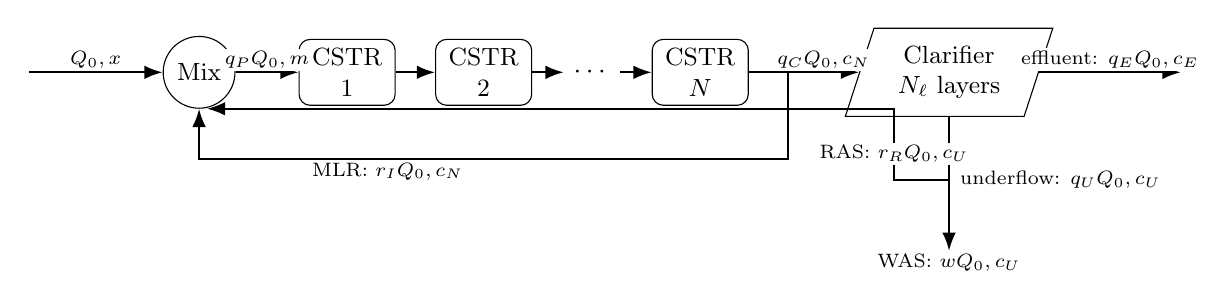
\begin{tikzpicture}[
  >=Latex,
  unit/.style={draw,rounded corners,minimum width=1.22cm,minimum height=0.72cm,align=center,font=\small},
  mix/.style={draw,circle,minimum size=0.83cm,align=center,font=\small},
  clar/.style={draw,trapezium,trapezium left angle=72,trapezium right angle=108,minimum width=1.55cm,minimum height=1.12cm,align=center,font=\small},
  stream/.style={->,thick},
  lab/.style={font=\scriptsize,fill=white,inner sep=1pt}
]
\node[mix] (mix) {Mix};
\node[unit,right=8mm of mix] (r1) {CSTR\\1};
\node[unit,right=5mm of r1] (r2) {CSTR\\2};
\node[right=4mm of r2] (dots) {$\cdots$};
\node[unit,right=4mm of dots] (rn) {CSTR\\$N$};
\coordinate[right=5mm of rn] (mlrsplit);
\node[clar,right=9mm of mlrsplit] (cl) {Clarifier\\$N_\ell$ layers};
\draw[stream] ([xshift=-17mm]mix.west) -- (mix.west) node[midway,above,lab] {$Q_0,x$};
\draw[stream] (mix) -- (r1) node[midway,above,lab] {$q_PQ_0,m$};
\draw[stream] (r1) -- (r2);
\draw[stream] (r2) -- (dots);
\draw[stream] (dots) -- (rn);
\draw[thick] (rn) -- (mlrsplit);
\draw[stream] (mlrsplit) -- (cl) node[midway,above,lab] {$q_CQ_0,c_N$};
\draw[stream] (mlrsplit) -- ++(0,-11mm) -| (mix.south) node[pos=0.34,below,lab] {MLR: $r_IQ_0,c_N$};
\draw[stream] (cl.east) -- ++(18mm,0) node[midway,above,lab] {effluent: $q_EQ_0,c_E$};
\draw[thick] (cl.south) -- ++(0,-8mm) coordinate (usplit);
\node[lab,right=1mm of usplit] {underflow: $q_UQ_0,c_U$};
\draw[stream] (usplit) -- ++(0,-9mm) node[below,lab] {WAS: $wQ_0,c_U$};
\draw[stream] (usplit) -- ++(-7mm,0) |- ([xshift=1mm]mix.south) node[pos=0.27,below,lab] {RAS: $r_RQ_0,c_U$};
\end{tikzpicture}
\caption{Stream-by-stream picture of the prescribed recycling $N$-stage activated sludge system. The MLR branch is taken before the Clarifier; RAS and WAS are hydraulic splits of one Clarifier underflow.}
\label{fig:process_schematic}
\end{figure}

The fresh flow $Q_0$ is a convenient common ruler for the three manipulated side streams. Define
\begin{equation}
\label{eq:flow_ratios}
r_I=\frac{Q_I}{Q_0},\qquad
r_R=\frac{Q_R}{Q_0},\qquad
w=\frac{Q_W}{Q_0},
\end{equation}
where $r_I$ is the MLR ratio, $r_R$ is the RAS ratio, and $w$ is the WAS ratio. The domain requires $r_I\geq0$, $r_R>0$, and $0\leq w<1$. These restrictions are not cosmetic: they keep every outlet flow and every concentration recovery division positive.

Starting at the mixer and following the arrows in Figure~\ref{fig:process_schematic} gives four dimensionless throughflows:
\begin{equation}
\label{eq:network_flows}
\underbrace{q_P}_{\text{through CSTRs}}=1+r_I+r_R,\qquad
\underbrace{q_C}_{\text{into Clarifier}}=1+r_R,
\qquad
\underbrace{q_U}_{\text{underflow}}=r_R+w,
\qquad
\underbrace{q_E}_{\text{effluent}}=1-w.
\end{equation}
The first identity counts fresh feed plus both returns. Removing MLR from the last-stage outlet leaves $q_CQ_0$. The Clarifier then divides that stream into $q_EQ_0$ and $q_UQ_0$, and the definitions show directly that $q_C=q_E+q_U$. This small hydraulic calculation is used repeatedly below; it is what makes RAS an internal stream and WAS an external loss.

Let $m$ denote the mixer outlet, $c_i$ the outlet of CSTR $i$, and $c_U$ the Clarifier underflow. The mass entering the first tank must equal the fresh-feed mass plus the two returned masses, component by component:
\begin{equation}
\label{eq:headworks_mixing}
q_Pm=x+r_Ic_N+r_Rc_U.
\end{equation}
Every term has the form ``flow relative to $Q_0$ times concentration.'' The factor $Q_0$ therefore cancels. Equation~\eqref{eq:headworks_mixing} is an identity, not a relationship to be learned. A topology with MLR withdrawn from another stage uses that stage state in place of $c_N$.

For a general prescribed topology, collect the stage volumes, aeration settings, and recycle decisions as
\begin{equation}
\label{eq:general_operating_vector}
\vartheta=
\left(\tau_1,\ldots,\tau_N,
a_1,\ldots,a_N,r_I,r_R,w\right)^\top\in\mathcal V,
\qquad
\tau_i=\frac{24V_i}{Q_0}.
\end{equation}
Here $\tau_i$ is the nominal HRT in hours that tank $i$ would provide at fresh flow alone. At fixed $Q_0$, choosing $\tau_i$ chooses volume, $V_i=Q_0\tau_i/24$; it is therefore a design decision, not merely an operating knob. The liquid actually traverses the tank at $q_PQ_0$, so its one-pass residence time and dilution rate are
\begin{equation}
\label{eq:recycle_hydraulics}
h_i=\frac{\tau_i}{q_P},
\qquad
\mathfrak d_i=\frac{24q_P}{\tau_i}\ \mathrm{d}^{-1}.
\end{equation}
An engineer can read Equation~\eqref{eq:recycle_hydraulics} directly: increasing either recycle while tank volume is fixed moves more water through the same vessel and shortens one pass. The surrogate must see this coupling because the biology does.

\subsection{From CSTR Balances to Inventory Rails}

The next task is to state the physical equations that the optimization must satisfy. For CSTR $i$, steady accumulation is zero, so the difference between outlet and inlet transport must be supplied by reactions and oxygen transfer:
\begin{equation}
\label{eq:stage_balance}
\mathfrak d_i(c_i-c_{i-1})=\nu^\top\varrho_i+\omega_i e_{S_O},
\qquad c_0=m.
\end{equation}
The $F$ entries of $c_i-c_{i-1}$ are component changes across the tank. The $P$ entries of $\varrho_i$ are the ASM2d-TSN process rates, and the columns of $\nu^\top$ translate those rates into component production or consumption. The last term adds oxygen through aeration; $e_{S_O}$ selects only the dissolved-oxygen coordinate.

The combined NLP carries a smooth form of this full rate vector, but invariant combinations remain valuable structural checks on the equations and reconstructed streams. Appendix~\ref{app:stoichiometry} constructs five physical conservation rows in $B$ and normalizes each row separately to form $A\in\R^{K\times F}$. Separate normalization keeps the inert-soluble, nitrogen, phosphorus, alkalinity, and metal inventories as recognizable rails. Its required checks are
\begin{equation}
\label{eq:invariant_conditions}
A\nu^\top=0,\qquad Ae_{S_O}=0,\qquad
\operatorname{rank}(A)=K,\qquad \|A_{k,:}\|_2=1.
\end{equation}
The first equality says that each row of $A$ annihilates every reaction source; the second prevents external oxygen transfer from masquerading as a conserved inventory; full row rank removes duplication, and the final relation fixes each rail's scale without mixing it with another inventory.

Premultiplying Equation~\eqref{eq:stage_balance} by $A$ removes both source terms. Because $\mathfrak d_i>0$, the remaining statement is simply
\begin{equation}
\label{eq:stage_invariants}
Ac_1=Am,\qquad
Ac_i=Ac_{i-1},\quad i=2,\ldots,N.
\end{equation}
These equalities are useful to picture as $K$ rails extending through the train: individual COD, nitrogen, phosphorus, and biomass components may move between forms, but the selected stoichiometric inventories cannot jump from one tank to the next. They need not equal $Ax$, because RAS changes the material circulating inside the plant. The fresh-feed relation appears only after the external Clarifier and WAS boundaries are closed.

\subsection{Following Components Through the Clarifier}

The Clarifier changes where material leaves, not how much of a non-reactive component exists. Its component balance is therefore
\begin{equation}
\label{eq:clarifier_balance_concentration}
q_Cc_N=q_Ec_E+q_Uc_U.
\end{equation}
The small underflow ratio can make $c_U$ numerically large even when its component mass is ordinary. It is more stable and more intuitive to predict the outlet masses normalized by fresh flow:
\begin{equation}
\label{eq:clarifier_mass_flow_coordinates}
g_E=q_Ec_E,\qquad g_U=q_Uc_U.
\end{equation}
Equation~\eqref{eq:clarifier_balance_concentration} then becomes
\begin{equation}
\label{eq:clarifier_balance}
g_E+g_U=q_Cc_N.
\end{equation}
Once $q_E$ and $q_U$ are known, the outlet concentrations are recovered uniquely as $c_E=g_E/q_E$ and $c_U=g_U/q_U$. Thus, non-negative mass-flow coordinates also give non-negative outlet concentrations.

Clarification must not be represented as solids generation. The TSS map satisfies $t_X\in\R_+^F$, $E_St_X=0$, and $\|t_X\|_1>0$. Once the development block $\mathcal D$ described below has been generated, define the frozen reporting scale
\begin{equation}
S_{f,j}=\max\!\left(1,\max_{i\in\mathcal D}|q_{C,i}c_{N,ij}|\right)
\end{equation}
in the tabulated mass-flow-coordinate unit. A particulate recovery is reported only when $q_Cc_{N,j}>10^{-10}S_{f,j}$. For such a coordinate define the underflow recovery and concentration ratio by
\begin{equation}
\label{eq:component_recovery}
\eta_j=\frac{g_{U,j}}{q_Cc_{N,j}},
\qquad
\upsilon_j=\frac{c_{U,j}}{c_{N,j}}
=\eta_j\frac{q_C}{q_U}.
\end{equation}
The first factor, $\eta_j$, is the fraction of incoming particulate mass sent downward. Non-negativity and Clarifier balance give $0\leq\eta_j\leq1$; the densification rule sharpens this to $q_U/q_C\leq\eta_j\leq1$ and therefore $1\leq\upsilon_j\leq q_C/q_U$. The factor $q_C/q_U$ expresses how recovered mass is concentrated into a smaller water stream. At or below the declared threshold, neither ratio is identifiable and it is reported as unavailable; the scale and availability flag are persisted.

The soluble and particulate coordinates require different physical rules. Let $E_S$ select the ten soluble components and $E_X$ the ten particulate components. Ideal soluble pass-through means that the underflow carries the same soluble concentration as the feed:
\begin{equation}
\label{eq:soluble_passthrough}
E_Sg_U=q_UE_Sc_N.
\end{equation}
Together with Equation~\eqref{eq:clarifier_balance}, this also gives $E_Sc_E=E_Sc_U=E_Sc_N$. For particulates, the mechanistic Clarifier moves a common floc solids flux. A successfully reconstructed and validated state must exhibit the physically necessary direction of that movement component by component:
\begin{equation}
\label{eq:particulate_densification}
E_Xg_U\geq q_UE_Xc_N.
\end{equation}
Equivalently, every particulate underflow concentration is at least its feed concentration. Because $g_E\geq0$ and Equation~\eqref{eq:clarifier_balance} holds, recovery cannot exceed the incoming particulate mass. In the combined formulation, these relationships follow from the layer-based component reconstruction when its physical profile is reproduced; they are replayed as diagnostics rather than introduced as substitute kinetic constraints.

A single learned Clarifier inventory would leave no way to verify where the solids reside. The response therefore contains the $N_\ell$ layer TSS concentrations
\begin{equation}
\label{eq:clarifier_layer_vector}
s=(s_1,\ldots,s_{N_\ell})^\top,
\end{equation}
ordered from the top water surface to the bottom hopper. The two end layers are tied to the outlet TSS values,
\begin{equation}
\label{eq:clarifier_endpoint_tss}
q_Es_1=t_X^\top g_E,
\qquad
q_Us_{N_\ell}=t_X^\top g_U,
\end{equation}
and an accepted exact state is checked against the physically interpretable top-to-bottom envelope,
\begin{equation}
\label{eq:clarifier_layer_envelope}
s_1\leq s_\ell\leq s_{N_\ell},
\qquad \ell=2,\ldots,N_\ell-1.
\end{equation}
The Clarifier solids inventory is now a consequence of a pictured profile rather than an independent output:
\begin{equation}
\label{eq:clarifier_inventory}
M_{\mathrm{cl}}=\sum_{\ell=1}^{N_\ell}V_{\mathrm{cl},\ell}s_\ell,
\qquad
\overline M_{\mathrm{cl}}=\frac{M_{\mathrm{cl}}}{Q_0}.
\end{equation}

The stream bookkeeping can now be closed around the entire plant. Premultiply the mixer balance by $A$, use the reactor rails in Equation~\eqref{eq:stage_invariants}, substitute the Clarifier balance, and cancel MLR and RAS because both remain inside the boundary. What remains is
\begin{equation}
\label{eq:plant_boundary_invariant}
Ax=q_EAc_E+wAc_U
=Ag_E+\frac{w}{q_U}Ag_U.
\end{equation}
This is the engineer's external check: conserved inventory enters only with fresh wastewater and leaves only with treated overflow and wasted sludge.

\subsection{One Identifiable Response for the Complete Loop}

Separate unit surrogates would have to be iterated around two recycle paths. Instead, collect every quantity needed to describe the closed loop in one response:
\begin{equation}
\label{eq:stacked_state}
\chi=
\begin{bmatrix}
m\\c_1\\\vdots\\c_N\\g_E\\g_U\\s
\end{bmatrix}
\in\R^L,
\qquad
L=(N+3)F+N_\ell.
\end{equation}
For the five-CSTR, 20-component, ten-layer case, $L=170$. Concentrations, normalized mass flows, and layer TSS have different units, so the regression is built in standardized coordinates. Let
\begin{equation}
\label{eq:standardized_inputs_states}
\widetilde\vartheta=S_\vartheta^{-1}(\vartheta-\mu_\vartheta),\qquad
\widetilde x=S_x^{-1}(x-\mu_x),\qquad
\widetilde\chi=D_\chi^{-1}(\chi-\mu_\chi),
\end{equation}
where all centers and positive diagonal scales come only from the development rows.

A second-order model needs squares and cross-products, but it needs each monomial only once. Let $q(v)$ list $v_jv_k$ for $j\leq k$, and form the nonconstant vector
\begin{equation}
\label{eq:unique_quadratic_terms}
\psi(\vartheta,x)=
\begin{bmatrix}
\widetilde\vartheta\\
\widetilde x\\
q(\widetilde\vartheta)\\
q(\widetilde x)\\
\widetilde\vartheta\otimes\widetilde x
\end{bmatrix}.
\end{equation}
Centering and scaling these nonconstant terms once more gives the serialized feature vector
\begin{equation}
\label{eq:system_feature_map}
\phi(\vartheta,x)=
\begin{bmatrix}
1\\S_\psi^{-1}[\psi(\vartheta,x)-\mu_\psi]
\end{bmatrix},
\qquad
d_\phi=1+n_\vartheta+F+\frac{n_\vartheta(n_\vartheta+1)}2+\frac{F(F+1)}2+n_\vartheta F.
\end{equation}
For $n_\vartheta=5$ and $F=20$, the basis contains $d_\phi=351$ columns. It includes every linear term, square, within-vector cross-product, and design--influent interaction exactly once. Within $q(v)$ the pairs are serialized lexicographically as $(1,1),(1,2),\ldots,(1,d),(2,2),\ldots,(d,d)$; the Kronecker block is serialized with the influent index varying fastest.

The frozen raw prediction is
\begin{equation}
\label{eq:raw_surrogate}
\widetilde\chi_{\mathrm{raw}}=\widehat C\phi(\vartheta,x),
\qquad
\widehat\chi(\vartheta,x)=\mu_\chi+D_\chi\widetilde\chi_{\mathrm{raw}}.
\end{equation}
The matrix $\widehat C\in\R^{L\times d_\phi}$ is the complete input--response map. Its design matrix must pass the full-column-rank and condition-number tests stated in the training procedure. For a fixed influent, Equation~\eqref{eq:raw_surrogate} is a vector-valued quadratic in the design and operating decisions.

\subsection{Reconstructing the Complete Response from Physical States}

The surrogate supplies a statistical center, but it does not supply the state variables used by the optimizer. Those variables are the $NF$ reactor concentrations and $N_\ell$ Clarifier-layer concentrations,
\begin{equation}
\label{eq:mechanistic_state}
y=(c_1^\top,\ldots,c_N^\top,s_1,\ldots,s_{N_\ell})^\top
\in\mathbb R_+^{NF+N_\ell}.
\end{equation}
For the case study, $y\in\mathbb R_+^{110}$. Given $(\vartheta,y,x)$, take $c_N$ directly from the final reactor block and set $s_F=t_X^\top c_N$. Soluble components pass through the Clarifier, while every particulate component follows the common layer-TSS proportions:
\begin{equation}
\label{eq:combined_outlet_reconstruction}
\begin{aligned}
c_{E,j}&=c_{U,j}=c_{N,j}, &&j\in\mathcal S,\\
c_{E,j}&=\frac{s_1}{s_F}c_{N,j},\qquad
c_{U,j}=\frac{s_{N_\ell}}{s_F}c_{N,j}, &&j\in\mathcal X.
\end{aligned}
\end{equation}
The optimization guard $s_F\geq1$ makes every displayed ratio well defined at a feasible point; a finite $C^2$ reciprocal extension used during infeasible trial evaluations is specified below. The remaining response blocks follow without another solve:
\begin{equation}
\label{eq:combined_response_reconstruction}
g_E=q_Ec_E,\qquad g_U=q_Uc_U,\qquad
m=\frac{x+r_Ic_N+r_Rc_U}{q_P},\qquad
\chi=\chi(\vartheta,y;x)
=\begin{bmatrix}m\\c_1\\\vdots\\c_N\\g_E\\g_U\\s\end{bmatrix}.
\end{equation}
This construction is the bridge between the 110-state physics and the 170-response statistics. It closes the mixer and Clarifier component balances, preserves soluble pass-through, and ties both outlet TSS concentrations and the Clarifier inventory to the layer profile. The reactor and layer balances introduced below then determine whether those reconstructed streams form a steady physical plant.

The statistical model is used as a calibrated feasibility envelope around this reconstructed response. Define
\begin{equation}
\label{eq:surrogate_fidelity}
d(\vartheta,x,y)=\frac{1}{L}
\left\|D_\chi^{-1}\left[\chi(\vartheta,y;x)-\widehat\chi(\vartheta,x)\right]\right\|_2^2.
\end{equation}
Here $D_\chi$ contains only development-set target scales. The calibration procedure later supplies a finite, strictly positive threshold $\delta$. Requiring $d\leq\delta$ keeps the physical state within the calibrated standardized neighborhood of the statistical center. It is a constraint, not an objective term. Split-conformal coverage applies to exchangeable future design rows and is not claimed for an optimizer-selected input.

\subsection{From a Physical State to an Engineering Decision}

The discharge is $c_E$, not the mixed liquor $c_N$. Let $T$ select the effluent components or composites to be scored, let $D_T$ contain frozen positive development-response scales, and let $\alpha_Q\geq0$ with $\mathbf1^\top\alpha_Q=1$. A dimensionless concentration-quality term is
\begin{equation}
\label{eq:quality_objective}
J_Q(\chi)=\alpha_Q^\top D_T^{-1}Tc_E
=\alpha_Q^\top D_T^{-1}T\frac{g_E}{q_E}.
\end{equation}
Concentration is used because the primary case represents discharge-quality limits; the corresponding loads $Q_0Tg_E$ are retained and reported separately. Let $J_{\mathrm{des/op}}$ contain the declared volume, aeration, pumping, and wasted-solids contributions. The complete engineering score is
\begin{equation}
\label{eq:network_objective}
J(\vartheta,\chi)=\lambda_QJ_Q(\chi)+J_{\mathrm{des/op}}(\vartheta,\chi),
\qquad \lambda_Q>0.
\end{equation}

Equipment and permit limits answer whether a simultaneous state may be operated. Denote the five engineering inequalities by $g_{\mathrm{eng}}(\vartheta,\chi)\leq0$. Whole-plant SRT is one such quantity. Because the Clarifier inventory is derived from the layer profile, it is
\begin{equation}
\label{eq:srt}
\mathrm{SRT}(\vartheta,\chi)=
\frac{\displaystyle\sum_{i=1}^{N}V_it_X^\top c_i+
\displaystyle\sum_{\ell=1}^{N_\ell}V_{\mathrm{cl},\ell}s_\ell}
{Q_0\left(q_Et_X^\top c_E+wt_X^\top c_U\right)}.
\end{equation}
The numerator is all suspended solids held in the CSTRs and Clarifier. The denominator contains only solids that cross the plant boundary in effluent and WAS. MLR and RAS are absent because they circulate internally. In the NLP, positive-solids domain guards are imposed before SRT is used, and the 8--30 d limits are written by cross multiplication. Consequently, the numerical formulation never divides by a trial-state boundary-solids loss.

Let $D_\vartheta=\diag(\vartheta^U-\vartheta^L)$ and normalize the five controls by
\begin{equation}
\label{eq:network_normalization}
z=D_\vartheta^{-1}(\vartheta-\vartheta^L)\in[0,1]^5.
\end{equation}
The normalized controls and the internally scaled physical states are the only optimization variables. The statistical response is never allowed to move independently of a mechanistic state: it is always the reconstruction $\chi[\vartheta(z),y;x]$. The full combined NLP is stated after its smooth mechanistic equations and numerical scales have been defined.

\subsection{Local-Solution Interpretation}

The raw surrogate is quadratic in $z$, while the flow-dependent balances contain products of controls and state coordinates. Kinetic rates, SRT restrictions, and Clarifier fluxes are nonlinear. The simultaneous problem is therefore nonconvex. Nine deterministic starts are solved independently, and only the best accepted local result is reported. No start, first-order certificate, or comparison among nine starts establishes global optimality.

\section{Methodology}

\subsection{End-to-End Study Design}

The computational study follows four information-separated phases. First, the coupled ASM2d-TSN--Clarifier model generates one fixed 20,000-state design. Second, three independently generated blocks provide 14,000 development rows, 2000 calibration rows, and 4000 assessment rows. The estimator, preprocessing, state scales, objective scales, and smooth-equation scales are fitted once using development rows only; calibration fixes $\delta$, and the untouched assessment rows gate the frozen raw response. Third, one combined physics-constrained statistical NLP is solved from nine deterministic starts for every nominal, robustness, and sensitivity case. Fourth, its one selected local candidate receives one exact nonsmoothed dynamic replay. Calibration, assessment, and optimization responses never refit the estimator or alter any scale, feature, weight, tolerance, or case definition.

\subsection{Coupled Reactor--Clarifier Data Generator}

The reaction model is ASM2d with two-step nitrification (ASM2d-TSN), comprising $P=28$ processes and $F=20$ components (Guerrero et al., 2011; Henze et al., 2006). Appendix~\ref{app:mechanistic_definition} gives every rate, stoichiometric coefficient, composition coefficient, and parameter value used here. Every matrix, prediction, and physical check uses the fixed order
\begin{equation}
\label{eq:component_order}
\begin{split}
(&S_O,S_F,S_A,S_{NH4},S_{NO2},S_{NO3},S_{N2},S_{PO4},S_I,S_{ALK},\\
&X_I,X_S,X_H,X_{PAO},X_{PP},X_{PHA},X_{AOB},X_{NOB},X_{MeP},X_{MeOH}).
\end{split}
\end{equation}
The first ten entries are soluble and the last ten particulate. Component units remain those of the mechanistic model; COD, TN, TP, and TSS are calculated only after a complete component state is available through the fixed $I_{\mathrm{comp}}$ matrix.

The case study fixes $N=5$ equal-volume CSTRs. CSTRs 1--2 are unaerated denitrification stages, CSTRs 3--5 share one manipulated aerobic intensity, and MLR is taken from CSTR 5. Appendix~\ref{app:stoichiometry} defines a deterministic five-row physical conservation matrix $B$ and its row-normalized form $A$. For a matrix $C\in\R^{m\times n}$ with singular values $\sigma_1\geq\sigma_2\geq\cdots$, define $\operatorname{rank}_\varepsilon(C)$ as the number satisfying $\sigma_k>\max(m,n)\varepsilon_{\mathrm{mach}}\sigma_1$. Generation stops unless $\operatorname{rank}_\varepsilon(\nu)=15$, $\operatorname{rank}_\varepsilon(B)=\operatorname{rank}_\varepsilon(A)=5$, and $\|A\nu^\top\|_\infty$, $\|Ae_{S_O}\|_\infty$, and $\max_k|\|A_{k,:}\|_2-1|$ are each no larger than $10^{-10}$.

The last CSTR feeds a non-reactive, one-dimensional $N_\ell=10$ layer Clarifier based on the flux-limited clarification--thickening model of Tak\'acs et al. (1991) and the benchmark conventions of Alex et al. (2018) and Jeppsson et al. (2007). To make the numerical generator reproducible, let $s_\ell$ be layer TSS, $s_F=t_X^\top c_5$ the feed TSS, and
\begin{equation}
\label{eq:settling_velocity}
v_s(s)=\max\!\left\{0,\min\!\left[v_0^{\max},
v_0\left(e^{-r_h(s-s_{\min})}-e^{-r_p(s-s_{\min})}\right)\right]\right\},
\qquad s_{\min}=f_{ns}s_F.
\end{equation}
The two exponentials describe hindered settling at high solids and the low-concentration branch; the outer bounds prevent a negative settling speed or a speed above $v_0^{\max}$. Define the unrestricted gravity flux $j_s(s)=v_s(s)s$. At the interface between top-to-bottom layers $\ell$ and $\ell+1$, the benchmark receiver-capacity limiter is
\begin{equation}
\label{eq:clarifier_flux_limiter}
j^{\mathrm{set}}_{\ell+1/2}=
\begin{cases}
j_s(s_\ell), & s_{\ell+1}\leq X_t,\\
\min\{j_s(s_\ell),j_s(s_{\ell+1})\}, & s_{\ell+1}>X_t.
\end{cases}
\end{equation}
This expression lets dilute receiving layers accept the incoming gravity flux and limits that flux when the receiving layer is already concentrated.

Take downward flux as positive and let the feed enter layer $\ell_F=5$ in a top-to-bottom, one-based array (the fifth layer from the top and sixth from the bottom). Above the feed, bulk liquid moves upward at $v_E=Q_0q_E/A_{\mathrm{cl}}$; below it, bulk liquid moves downward at $v_U=Q_0q_U/A_{\mathrm{cl}}$. The total internal-interface TSS flux is therefore
\begin{equation}
\label{eq:clarifier_total_flux}
\mathcal J_{\ell+1/2}=
\begin{cases}
-v_Es_{\ell+1}+j^{\mathrm{set}}_{\ell+1/2}, & \ell<\ell_F,\\
v_Us_\ell+j^{\mathrm{set}}_{\ell+1/2}, & \ell\geq\ell_F.
\end{cases}
\end{equation}
At the water surface and hopper, $\mathcal J_{1/2}=-v_Es_1$ and $\mathcal J_{N_\ell+1/2}=v_Us_{N_\ell}$; no gravity flux is allowed to cross those physical boundaries. The finite-volume layer balance is
\begin{equation}
\label{eq:clarifier_layer_balance}
V_{\mathrm{cl},\ell}\frac{ds_\ell}{dt}
=A_{\mathrm{cl}}(\mathcal J_{\ell-1/2}-\mathcal J_{\ell+1/2})
\,+\,\mathbf1_{\{\ell=\ell_F\}}Q_0q_Cs_F.
\end{equation}
Summing Equation~\eqref{eq:clarifier_layer_balance} over all layers cancels internal fluxes and recovers $q_Cs_F=q_Es_1+q_Us_{N_\ell}$ at steady state. This is why the endpoint equations in the simultaneous physical constraints are not arbitrary additions.

Soluble components follow the liquid phase unchanged. Particulate components share the TSS flux and retain the Clarifier-feed particulate proportions. The complete layer reconstruction is
\begin{equation}
\label{eq:clarifier_component_reconstruction}
c_{\mathrm{cl},\ell,j}=
\begin{cases}
c_{5,j},&j\in\mathcal S,\\
(c_{5,j}/s_F)s_\ell,&j\in\mathcal X,\ s_F>0,\\
0,&j\in\mathcal X,\ s_F=0,
\end{cases}
\qquad
\mathcal J_{\ell+1/2,j}=(c_{5,j}/s_F)\mathcal J_{\ell+1/2}
\quad(j\in\mathcal X, s_F>0).
\end{equation}
Thus $c_{E,j}=(c_{5,j}/s_F)s_1$ and $c_{U,j}=(c_{5,j}/s_F)s_{N_\ell}$ for particulates. Because every particulate entry of $t_X$ is positive, $s_F=0$ in a non-negative state implies that all particulate feed coordinates are zero, so the limiting definition is mass consistent.

\begin{table}[htbp]
\centering
\caption{Fixed multilayer-Clarifier geometry and settling parameters.}
\label{tab:clarifier_parameters}
\scriptsize
\begin{tabular}{lll}
\toprule
Quantity & Value & Unit or convention \\
\midrule
Surface area $A_{\mathrm{cl}}$ & 1500 & m$^2$ \\
Total depth & 4.0 & m \\
Layer count; depth; volume & 10; 0.4; 600 & --; m; m$^3$ \\
Feed layer & 5 from top & 6 from bottom; array index 4 \\
Maximum settling speed $v_0^{\max}$ & 250 & m d$^{-1}$ \\
Theoretical coefficient $v_0$ & 474 & m d$^{-1}$ \\
Hindered coefficient $r_h$ & 0.000576 & m$^3$ g$^{-1}$ \\
Low-concentration coefficient $r_p$ & 0.00286 & m$^3$ g$^{-1}$ \\
Non-settleable fraction $f_{ns}$ & 0.00228 & dimensionless \\
Flux-limiting threshold $X_t$ & 3000 & g TSS m$^{-3}$ \\
Blanket diagnostic threshold & 3000 & g TSS m$^{-3}$ \\
\bottomrule
\end{tabular}
\end{table}

The mechanistic dynamic state is $y=(c_1,\ldots,c_5,s_1,\ldots,s_{10})\in\R_+^{110}$. At every residual evaluation, Equation~\eqref{eq:clarifier_component_reconstruction} gives $c_E$ and $c_U$, and Equation~\eqref{eq:headworks_mixing} gives $m$. The transient reactor balance whose steady form is Equation~\eqref{eq:stage_balance} is
\begin{equation}
\label{eq:reactor_dynamic_balance}
\frac{dc_i}{dt}=\mathfrak d_i(c_{i-1}-c_i)+\nu^\top\varrho(c_i)+\omega_i e_{S_O},
\qquad c_0=m.
\end{equation}
The five vector derivatives in Equation~\eqref{eq:reactor_dynamic_balance} and the ten scalar layer derivatives in Equation~\eqref{eq:clarifier_layer_balance} therefore form one coupled function $\dot y=\mathcal F_{\mathrm{dyn}}(y;\vartheta,x)$. Eliminating the mixer and outlet algebraic variables in this way does not break the loop: a change in the bottom layer immediately changes RAS, the mixer, CSTR 1, and every downstream state in the same residual evaluation.

The nonlinear residual is expressed in dimensionless-state rates. Reactor component $(i,j)$ is divided by $c_j^{\mathrm{ref}}=\max(1,x_j^U)$, where $x_j^U$ is the upper bound in Table~\ref{tab:influent_ranges}; every layer derivative uses one fixed start-specific reference $s_0^{\mathrm{ref}}=\max[1,t_X^\top c_5(y_0)]$. These values form the positive diagonal dynamic scale $S_{\mathrm{dyn}}$. The scaled derivative replay used for steady-state acceptance evaluates the same component references and the current Clarifier-feed TSS reference. This scaling gives one tolerance the same engineering meaning for dissimilar quantities such as dissolved oxygen and sludge-blanket solids.

Two initial states are prescribed. Start 1 uses $c_i=x$ for every stage and $s_\ell=t_X^\top x$ for every layer. Start 2 uses
\begin{equation}
c_i=E_S^\top E_Sx+\alpha_iE_X^\top E_Xx,
\quad (\alpha_1,\ldots,\alpha_5)=(1.5,2.0,2.5,3.0,3.5),
\end{equation}
and, after forming $s_F=t_X^\top c_5$,
\begin{equation}
(s_1,\ldots,s_{10})=s_F(0.002,0.005,0.01,0.03,0.10,0.50,1.25,2.25,3.25,4.00).
\end{equation}
Each prescribed initial state $y_0$ is first relaxed in scaled coordinates by integrating
\begin{equation}
\frac{d\widetilde y}{dt}=S_{\mathrm{dyn}}^{-1}\mathcal F_{\mathrm{dyn}}(S_{\mathrm{dyn}}\widetilde y;\vartheta,x),
\qquad \widetilde y(0)=S_{\mathrm{dyn}}^{-1}y_0,
\end{equation}
with variable-order BDF. The relaxation horizon follows the slow solids-removal mode,
\begin{equation}
T_{\mathrm{rel}}=\max(400,50/w)\ \mathrm{d},
\end{equation}
and the adaptive maximum step is $T_{\mathrm{rel}}/100$. The factor $50/w$ gives the slow solids mode enough time to satisfy both the local derivative and accumulated plant-boundary closure tests as wasting approaches its lower bound; it is an upper limit, not a forced simulation duration. Integration terminates early when the scaled derivative infinity norm reaches $10^{-9}$ d$^{-1}$. Relative and scaled-coordinate absolute tolerances are $10^{-7}$ and $10^{-9}$.

A successful integrator status is not by itself a positivity certificate. Every stored physical state on the scaled-state trajectory is checked and must be strictly positive. If an internal evaluation fails or any stored state is non-positive, the same start is retried with
\begin{equation}
y^{\log}=\log\widetilde y,
\qquad
\frac{dy^{\log}}{dt}=\diag(e^{y^{\log}})^{-1}S_{\mathrm{dyn}}^{-1}
\mathcal F_{\mathrm{dyn}}(S_{\mathrm{dyn}}e^{y^{\log}};\vartheta,x),
\end{equation}
which keeps every evaluated physical state on that route positive without clipping. The relaxed endpoint is replayed against the complete $10^{-8}$ acceptance contract below. Only an endpoint that misses that contract is supplied to a non-negative bounded trust-region-reflective least-squares calculation as a local polish, using \texttt{xtol}=\texttt{ftol}=\texttt{gtol}=$10^{-9}$ and at most 5000 residual evaluations. Start 1 fixes the branch when this complete route is accepted; Start 2 is used only after the complete Start-1 route fails. No preceding Latin-hypercube solution initializes another row.

For the stability screen, the reduced Jacobian is $J_y=\partial\mathcal F_{\mathrm{dyn}}/\partial y$ after the algebraic quantities have been eliminated. Column $j$ is calculated by a centered finite difference with step $\sqrt{\varepsilon_{\mathrm{mach}}}\max(1,|y_j|)$, using a forward difference only when the centered step would cross zero. The prescribed initialization route defines the mechanistic branch represented in the data; neither simultaneous NLP is assumed to make that nonlinear branch unique.

\begin{table}[htbp]
\centering
\caption{Mechanistic steady-state numerical and physical acceptance contract.}
\label{tab:mechanistic_acceptance}
\scriptsize
\begin{tabular}{lll}
\toprule
Check or setting & Limit & Purpose \\
\midrule
Nonlinear \texttt{xtol}, \texttt{ftol}, \texttt{gtol} & $10^{-9}$ & Steady nonlinear solve \\
Maximum residual evaluations & 5000 per start & Bounded retry effort \\
BDF relative; scaled absolute tolerance & $10^{-7}$; $10^{-9}$ & Dynamic relaxation \\
BDF horizon; maximum step & $T_{\mathrm{rel}}=\max(400,50/w)$ d; $T_{\mathrm{rel}}/100$ & WAS-scaled relaxation limit \\
Scaled CSTR/layer derivative & $\leq10^{-8}$ d$^{-1}$ & Local balance closure \\
Scaled early-stop derivative & $\leq10^{-9}$ d$^{-1}$ & Early terminal event before full replay \\
Minimum state coordinate & $\geq-10^{-10}$ & No clipped negative state \\
Largest real reduced-Jacobian eigenvalue & $\leq10^{-8}$ d$^{-1}$ & Local stability screen \\
Component Clarifier and plant-boundary residual & $\leq10^{-8}$ scaled & External closure \\
\bottomrule
\end{tabular}
\end{table}
For every algebraic balance written as $\sum_k t_k=0$, its scaled replay residual is $|\sum_k t_k|/\max(1,\sum_k|t_k|)$. The $10^{-8}$ external-closure limit in Table~\ref{tab:mechanistic_acceptance} applies to this quantity. Every accepted state also passes hydraulic splits, RAS/WAS common composition, soluble pass-through, $q_U/q_C-10^{-10}\leq\eta_j\leq1+10^{-10}$ for every available particulate ratio, the layer envelope, and finite-rate checks. The lower recovery bound is the mechanistic counterpart of $c_{U,j}\geq c_{5,j}$ and makes an accepted target feasible for the simultaneous-state inequalities to the stated tolerance. Every $\rho_p$, oxygen-transfer term, settling velocity, and interface flux must be finite and no smaller than $-10^{-12}$ when its mathematical definition is non-negative. A violation invalidates the state; negative quantities are not clipped into acceptance.

\subsection{Case-Study Design, Operating, and Influent Domains}

The primary case reduces the general vector in Equation~\eqref{eq:general_operating_vector} to five decisions:
\begin{equation}
\label{eq:case_operating_vector}
\vartheta=(H,a,r_I,r_R,w)^\top.
\end{equation}
The total nominal HRT is divided equally, so $\tau_i=H/5$ and $V_i=Q_0H/(24\times5)$. Aeration is zero in CSTRs 1--2 and $k_La=47a$ d$^{-1}$ in CSTRs 3--5. Table~\ref{tab:network_domain} is both the training and optimization box; no surrogate response outside it is scored.

\begin{table}[htbp]
\centering
\caption{Fixed topology, joint design-and-operation domain, and engineering screens.}
\label{tab:network_domain}
\scriptsize
\begin{tabular}{lll}
\toprule
Quantity & Value or range & Interpretation \\
\midrule
Fresh flow $Q_0$ & $10{,}000$ m$^3$ d$^{-1}$ & Plant throughput basis \\
Number of CSTRs $N$ & 5 & Fixed topology \\
Nominal total HRT $H$ & $[6,36]$ h & Sets five equal tank volumes \\
Aerobic setting $a$ & $[0,1]$ & $k_La=47a$ d$^{-1}$ in CSTRs 3--5 \\
MLR ratio $r_I$ & $[0,4]$ & $Q_I/Q_0$ \\
RAS ratio $r_R$ & $[0.25,1.25]$ & $Q_R/Q_0$ \\
WAS ratio $w$ & $[0.001,0.05]$ & $Q_W/Q_0$ \\
Dissolved-oxygen saturation & 8.5 g O$_2$ m$^{-3}$ & Aeration boundary \\
SRT acceptance interval & $[8,30]$ d & Engineering capacity constraint \\
Clarifier surface overflow & $\leq20$ m d$^{-1}$ & Engineering hydraulic screen \\
Clarifier feed solids loading & $\leq100$ kg TSS m$^{-2}$ d$^{-1}$ & Engineering solids screen \\
Underflow TSS $X_U^{\max}$ & $\leq15{,}000$ g TSS m$^{-3}$ & Pumpability screen \\
\bottomrule
\end{tabular}
\end{table}

The surface-overflow and solids-loading screens are
\begin{equation}
\label{eq:clarifier_loadings}
\mathrm{SOR}=\frac{Q_0q_E}{A_{\mathrm{cl}}},
\qquad
\mathrm{SLR}=\frac{Q_0q_Ct_X^\top c_5}{1000A_{\mathrm{cl}}}.
\end{equation}
The factor 1000 converts grams to kilograms in SLR. These are case-study engineering screens (Tchobanoglous et al., 2014), not fitted Tak\'acs parameters. At fixed $Q_0$ and area, SOR cannot become active over the declared WAS range but is retained as a hydraulic safety check. The primary underflow-TSS limit is 15,000 g TSS m$^{-3}$; the precisely matched 12,000 and 20,000 g TSS m$^{-3}$ sensitivity cases are defined with the objective-weight cases below.

Table~\ref{tab:influent_ranges} completes the 25-dimensional training domain. The alkalinity range is expressed in the ASM unit mol HCO$_3^-$ m$^{-3}$: 80--260 g CaCO$_3$ m$^{-3}$ converts to 1.6--5.2 mol of charge m$^{-3}$, which is the range used in the component vector.

\begin{table}[htbp]
\centering
\caption{Fresh-influent component ranges for mechanistic design and surrogate fitting.}
\label{tab:influent_ranges}
\scriptsize
\begin{tabular}{llllll}
\toprule
Component & Range & Unit & Component & Range & Unit \\
\midrule
$S_O$ & $[0.0,0.5]$ & g O$_2$ m$^{-3}$ & $S_I$ & $[10,90]$ & g COD m$^{-3}$ \\
$S_F$ & $[20,180]$ & g COD m$^{-3}$ & $S_{ALK}$ & $[1.6,5.2]$ & mol HCO$_3^-$ m$^{-3}$ \\
$S_A$ & $[5,80]$ & g COD m$^{-3}$ & $X_I$ & $[20,120]$ & g COD m$^{-3}$ \\
$S_{NH4}$ & $[12,55]$ & g N m$^{-3}$ & $X_S$ & $[60,280]$ & g COD m$^{-3}$ \\
$S_{NO2}$ & $[0,3]$ & g N m$^{-3}$ & $X_H$ & $[15,100]$ & g COD m$^{-3}$ \\
$S_{NO3}$ & $[0,8]$ & g N m$^{-3}$ & $X_{PAO}$ & $[5,60]$ & g COD m$^{-3}$ \\
$S_{N2}$ & $[0,2]$ & g N m$^{-3}$ & $X_{PP}$ & $[2,20]$ & g P m$^{-3}$ \\
$S_{PO4}$ & $[2,18]$ & g P m$^{-3}$ & $X_{PHA}$ & $[1,30]$ & g COD m$^{-3}$ \\
 & & & $X_{AOB}$ & $[0.5,8]$ & g COD m$^{-3}$ \\
 & & & $X_{NOB}$ & $[0.5,8]$ & g COD m$^{-3}$ \\
 & & & $X_{MeP}$ & $[0,12]$ & g TSS m$^{-3}$ \\
 & & & $X_{MeOH}$ & $[0,12]$ & g TSS m$^{-3}$ \\
\bottomrule
\end{tabular}
\end{table}

The nominal influent is the componentwise midpoint of Table~\ref{tab:influent_ranges}, in the order of Equation~\eqref{eq:component_order}:
\begin{equation}
\label{eq:nominal_influent}
\begin{split}
x_{\mathrm{nom}}=(&0.25,100,42.5,33.5,1.5,4,1,10,50,3.4,\\
&70,170,57.5,32.5,11,15.5,4.25,4.25,6,6)^\top.
\end{split}
\end{equation}
It is a designed in-domain influent, not a measured plant sample. Over the declared box,
\begin{equation}
q_P\in[1.25,6.25],\qquad H/5\in[1.2,7.2]\ \mathrm{h},\qquad
H/(5q_P)\in[0.192,5.76]\ \mathrm{h}.
\end{equation}
These are derived hydraulic supports of the joint design rather than additional acceptance constraints.

\subsection{Mechanistic Design and Stored Targets}

The stored design concatenates three independently generated blocks in the fixed 25-dimensional order $(H,a,r_I,r_R,w,x_1,\ldots,x_{20})$: a 14,000-point strength-1 Latin-hypercube development block (McKay et al., 1979), a 2000-point iid-uniform calibration block, and a 4000-point iid-uniform assessment block. Their separate SplitMix64 scalar states start at 42, 43, and 44, respectively. The random streams are defined here so that no software-specific seeding convention is required. All generator variables are unsigned 64-bit integers; $\oplus$ is bitwise exclusive-or, $\gg$ is a logical right shift, and every addition and multiplication is reduced modulo $2^{64}$. From the applicable block state $\mathsf q_0$, draw the word $\mathcal U_t$ by
\begin{align}
\mathsf q_{t+1}&=\mathsf q_t+\mathtt{9E3779B97F4A7C15}_{16},\\
\mathsf v_1&=[\mathsf q_{t+1}\oplus(\mathsf q_{t+1}\gg30)]\,\mathtt{BF58476D1CE4E5B9}_{16},\\
\mathsf v_2&=[\mathsf v_1\oplus(\mathsf v_1\gg27)]\,\mathtt{94D049BB133111EB}_{16},\\
\mathcal U_t&=\mathsf v_2\oplus(\mathsf v_2\gg31).
\end{align}
The draw counter advances once for every generated word, including a rejected shuffle word. For development dimension $j$, initialize $\pi_j=(0,\ldots,n_D-1)$ with $n_D=14{,}000$. For the separate shuffle index $k=n_D-1,\ldots,1$, let $b=k+1$ and $L_b=2^{64}-(2^{64}\bmod b)$; draw until $\mathcal U_t<L_b$ and swap entries $k$ and $\mathcal U_t\bmod b$. Here $L_b$ is an exact mathematical integer, permitted to equal $2^{64}$ and therefore exempt from the unsigned-64-bit storage statement; generator states and generated words remain unsigned 64-bit integers. This preserves the stated rejection sequence and is unbiased because $L_b$ is divisible by $b$. After that Fisher--Yates permutation, draw once for each development row in increasing order and set $\xi_{ij}=(\mathcal U_t\gg11)/2^{53}$. The development coordinate is
\begin{equation}
\zeta_{ij}=\frac{\pi_j(i-1)+\xi_{ij}}{n_D},\qquad i=1,\ldots,n_D.
\end{equation}
For calibration and assessment, reset to the block's stated seed, traverse rows first and the displayed dimensions second, draw exactly one word per coordinate, and set
\begin{equation}
\zeta_{ij}^{\mathrm{iid}}=
\frac{(\mathcal U_t\gg12)+1/2}{2^{52}}\in(0,1).
\end{equation}
The 52-bit midpoints are exactly representable in binary64, including the largest value $1-2^{-53}$, so no iid coordinate lies on a box face. Affine range maps send all unit coordinates to physical variables. Conditional on the development block, the calibration rows and a future iid-uniform row are exchangeable; the independent assessment block is untouched by fitting and calibration. Every point must produce an accepted state under Table~\ref{tab:mechanistic_acceptance}. A failed point is not replaced. If any point remains unresolved after the fixed retry route, the study stops without a fitted response. All generator states, draw counts, start attempts, and diagnostics are retained. The robustness design uses its separate stream stated later.

For each accepted row, the target vector is
\begin{equation}
\label{eq:mechanistic_target}
\chi_{\mathrm{ASM}}=
(m,c_1,\ldots,c_5,g_E,g_U,s_1,\ldots,s_{10})\in\R^{170}.
\end{equation}
The full component state of every Clarifier layer, $c_E$, $c_U$, component and TSS recoveries, composites, loadings, SRT, reaction and oxygen-transfer rates, initialization route, stability result, residuals, and solve time are retained as diagnostics. Outlet mass flows are modeled because their scale remains well behaved when $q_U$ is small; the layer TSS values make $M_{\mathrm{cl}}$ a derived quantity through Equation~\eqref{eq:clarifier_inventory}.

The three blocks retain their immutable concatenated order. Rows 1--14,000 form $\mathcal D$, rows 14,001--16,000 form $\mathcal C$, and rows 16,001--20,000 form $\mathcal A$. This 70/10/20 membership is fixed before any response is examined. Only $\mathcal D$ may determine preprocessing, scales, coefficients, and numerical row scales. Set $\mathcal C$ is used only once to fix $\delta$, and $\mathcal A$ remains untouched until the frozen estimator and threshold have been sealed. No row outside $\mathcal D$ enters a refit, and no candidate model is selected.

Two smaller profiles exercise the same block-generation, fitting, and combined-NLP contracts before the full study. The unit profile has 600 newly generated rows in three independent blocks, partitioned as 420 development, 60 calibration, and 120 assessment rows, with seeds 60042, 60043, and 60044; 420 exceeds the 351 feature columns. It evaluates 14 cases, attempts $9(14)=126$ combined-NLP starts, and requires at most $600+14=614$ BDF routes. The \texttt{test\_2000} profile has 1400, 200, and 400 rows with seeds 200042, 200043, and 200044, respectively, and runs ten robustness cases in addition to the nominal and 12 sensitivity cases. It therefore evaluates 23 cases, attempts $9(23)=207$ combined-NLP starts, and requires at most $2000+23=2023$ BDF routes. Each profile regenerates its three blocks at its declared sizes and profile-specific seeds; it is not an ordered prefix or subsample of the full design. These profiles verify execution only and do not contribute numerical results to the full-study tables.

\subsection{Fixed Development-Only Multiresponse Least-Squares Estimator}

For the fixed fitting set $\mathcal I=\mathcal D$, containing $n=14{,}000$ rows, define the population mean, population standard deviation, and numerical reference magnitude of a scalar coordinate $v$ by
\begin{equation}
\label{eq:fit_coordinate_scale}
\overline v_{\mathcal I}=\frac1n\sum_{i\in\mathcal I}v_i,
\quad
s_{\mathcal I}(v)=\left[\frac1n\sum_{i\in\mathcal I}(v_i-\overline v_{\mathcal I})^2\right]^{1/2},
\quad
a_{\mathcal I}(v)=\max\!\left(1,\max_{i\in\mathcal I}|v_i|\right).
\end{equation}
A coordinate is numerically variable only when
\begin{equation}
\label{eq:nonzero_variance_rule}
s_{\mathcal I}(v)>10^{-12}a_{\mathcal I}(v).
\end{equation}
This rule is applied to every design coordinate, influent coordinate, nonconstant monomial, and target coordinate. All 350 nonconstant feature coordinates and all 170 target coordinates must pass; the leading constant feature is retained by definition. Otherwise the fit is invalid.

The scaling matrices used throughout are fixed explicitly by the development rows:
\begin{equation}
\begin{aligned}
S_\vartheta&=\operatorname{Diag}\{s_{\mathcal D}(\vartheta_j)\},&
S_x&=\operatorname{Diag}\{s_{\mathcal D}(x_j)\},\\
S_\psi&=\operatorname{Diag}\{s_{\mathcal D}(\psi_j)\},&
D_\chi&=\operatorname{Diag}\{s_{\mathcal D}(\chi_j)\}.
\end{aligned}
\end{equation}
The corresponding $\mu_\vartheta,\mu_x,\mu_\psi,\mu_\chi$ are the development means in Equation~\eqref{eq:fit_coordinate_scale}, and $s_{\chi,j}:=s_{\mathcal D}(\chi_j)=(D_\chi)_{jj}$. No later block changes these matrices or centers.

Using only rows in $\mathcal I$, construct all centers and scales in Equations~\eqref{eq:standardized_inputs_states}--\eqref{eq:system_feature_map}. Let $Y_{\mathcal I}$ contain the mechanistic targets from Equation~\eqref{eq:mechanistic_target}, in the same row order as the features. The fitting matrices are
\begin{equation}
\label{eq:training_matrices}
\Phi_{\mathcal I}=\begin{bmatrix}\phi_1^\top\\\vdots\\\phi_n^\top\end{bmatrix}\in\R^{n\times d_\phi},
\qquad
\widetilde Y_{\mathcal I}=(Y_{\mathcal I}-\mathbf1_n\mu_\chi^\top)D_\chi^{-1}\in\R^{n\times L},
\end{equation}
where $d_\phi=351$ and $L=170$. The fixed estimator is
\begin{equation}
\label{eq:training_objective}
\widehat C_{\mathcal I}=\argminop_{C\in\R^{L\times d_\phi}}
\frac{1}{nL}\left\|\widetilde Y_{\mathcal I}-\Phi_{\mathcal I}C^\top\right\|_F^2.
\end{equation}
Every output is estimated from the single fixed standardized design in Equation~\eqref{eq:training_matrices}. There is no regularization choice, response-specific feature selection, hyperparameter search, or later refit.

A thin singular-value decomposition
\begin{equation}
\label{eq:design_svd}
\Phi_{\mathcal I}=U\Sigma V^\top,
\qquad \sigma_1\geq\cdots\geq\sigma_{d_\phi}\geq0,
\end{equation}
defines
\begin{equation}
\label{eq:design_rank_condition}
\tau_{\mathrm{rank}}=\max(n,d_\phi)\varepsilon_{\mathrm{mach}}\sigma_1,
\qquad
\kappa_2(\Phi_{\mathcal I})=\frac{\sigma_1}{\sigma_{d_\phi}}.
\end{equation}
The design is admissible only when
\begin{equation}
\label{eq:design_acceptance}
\sigma_{d_\phi}>\tau_{\mathrm{rank}},
\qquad
\kappa_2(\Phi_{\mathcal I})\leq10^8.
\end{equation}
Under these conditions Equation~\eqref{eq:training_objective} has one unique least-squares minimizer supported by the observed design.

The coefficients are calculated by column-pivoted Householder QR,
\begin{equation}
\Phi_{\mathcal I}\Pi=QR_\Phi,
\qquad
\widehat C_{\mathcal I}^{\top}=W_{\mathrm{QR}}
=\Pi R_\Phi^{-1}Q^\top\widetilde Y_{\mathcal I}.
\end{equation}
The triangular solution is followed by one iterative-refinement replay in the same factorization. With $R_Y^{(0)}=\Phi_{\mathcal I}W_{\mathrm{QR}}-\widetilde Y_{\mathcal I}$, solve
\begin{equation}
\Delta W=\Pi R_\Phi^{-1}Q^\top(-R_Y^{(0)}),
\qquad W_{\mathrm{QR}}\leftarrow W_{\mathrm{QR}}+\Delta W.
\end{equation}
This correction does not change the least-squares estimator; it suppresses triangular-solve roundoff before the normal-equation audit, which is especially important when a response is reproduced nearly exactly.
The independent SVD calculation is
\begin{equation}
W_{\mathrm{SVD}}=V\Sigma^{-1}U^\top\widetilde Y_{\mathcal I}.
\end{equation}
With $R_Y=\Phi_{\mathcal I}W_{\mathrm{QR}}-\widetilde Y_{\mathcal I}$, define
\begin{equation}
\label{eq:coefficient_acceptance}
\eta_{\mathrm{opt}}=
\frac{\|\Phi_{\mathcal I}^\top R_Y\|_F}
{\max\{1,\|\Phi_{\mathcal I}\|_2\|R_Y\|_F\}},
\quad
\eta_{\mathrm{agree}}=
\frac{\|W_{\mathrm{QR}}-W_{\mathrm{SVD}}\|_F}
{\max(1,\|W_{\mathrm{SVD}}\|_F)},
\quad
\max(\eta_{\mathrm{opt}},\eta_{\mathrm{agree}})
\leq100\kappa_2(\Phi_{\mathcal I})\varepsilon_{\mathrm{mach}}.
\end{equation}
All coefficients must also be finite. Failure of Equations~\eqref{eq:nonzero_variance_rule}, \eqref{eq:design_acceptance}, or \eqref{eq:coefficient_acceptance} invalidates the response; no alternate estimator is substituted.

The development rows also determine the mechanistic residual and smoothing scales defined with the combined NLP below. They are calculated from named physical terms rather than from nearly zero fitted residuals, then frozen before calibration, assessment, or optimization is opened.

\subsection{Computational Feasibility Gate}

The full study has 113 cases: one nominal case, 100 fresh-influent robustness cases, two additional underflow-TSS cases, and ten objective-weight cases. Each case uses nine starts of the single combined NLP. Define the complete logical workloads for one uninterrupted execution
\begin{equation}
\begin{aligned}
N_{\mathrm{BDF}}^{\max}&=20{,}000+113=20{,}113,\\
N_{\mathrm{combined\text{-}NLP}}^{\mathrm{sci}}&=9(113)=1017.
\end{aligned}
\end{equation}
The first term in $N_{\mathrm{BDF}}^{\max}$ is data generation. The remaining term reserves one independent replay for the selected combined-NLP result in every case. This is the planned logical maximum for uninterrupted completion: a case with no accepted NLP result has no decision to replay, so its realized logical count is smaller and is reported. An invocation counts once even when the prescribed internal Start-1/conditional-Start-2 generator route is needed. An interruption after a numerical call begins but before its completed record is committed can require a new physical attempt, so the actual attempt count can exceed this logical maximum; the invocation ledger described below makes that distinction explicit.

The first 256 design rows are executed as an uncontended serial timing preflight while remaining part of the immutable design; their complete-route times define $t_{\mathrm{BDF},95}$ by the nearest-rank rule. After calibration and assessment pass, a fixed case panel preflights and caches every one of the nine combined-NLP starts. The full and \texttt{test\_2000} panels contain the nominal case, all 12 nominal-influent sensitivity cases, and ten robustness influents, for 23 cases. The unit panel contains the same nominal and sensitivity cases and its one robustness influent, for 14 cases. When more than ten robustness influents are available, standardize their 20 coordinates by the configured spans, initialize the comparison set with the nominal influent, and repeatedly add the unselected robustness row maximizing its minimum Euclidean distance to the nominal and already selected rows. An exact tie uses the smaller original robustness-row index; selection stops at ten or when all available rows have been used.

Each completed combined-NLP start is an atomic checkpoint identified by profile, case, ordered start, and the exact scientific-contract hash. Its record is written completely, validated, hashed, and only then atomically committed. On resume, a checkpoint is reused only after its identity, contract hash, payload hash, dimensions, and finite-value requirements have been verified; a missing or unverifiable checkpoint is attempted anew and is never partially loaded. The selected candidate's exact BDF replay uses the same atomic and verified-reuse contract. A durable invocation ledger records every numerical attempt, its logical identity and attempt number, start and completion status, and whether a verified prior result was reused. Consequently, reports distinguish the planned logical workload, realized logical results, actual physical attempts including post-interruption reattempts, and verified cache reuses.

The nearest-rank 95th percentile over the panel's per-start durations defines $t_{\mathrm{NLP},95}$. Panel results are scientific results and are reused rather than rerun. With the observed one-time fit duration $t_{\mathrm{fit}}$, the empirical single-thread projection is
\begin{equation}
\label{eq:computational_projection}
T_{\mathrm{proj}}=t_{\mathrm{fit}}
+1.5\!\left[
20{,}113t_{\mathrm{BDF},95}
+1017t_{\mathrm{NLP},95}
\right].
\end{equation}
If $M_{\mathrm{fit}}$, $M_{\mathrm{BDF}}$, and $M_{\mathrm{NLP}}$ are the resident-set high-water marks observed over the complete fit, BDF-preflight, and NLP-preflight stages, respectively, set
\begin{equation}
M_{\mathrm{proj}}=1.5\max(M_{\mathrm{fit}},M_{\mathrm{BDF}},M_{\mathrm{NLP}}).
\end{equation}
The factor 1.5 is a declared safety factor applied to both timed workloads and observed memory. Proceeding beyond each preflight requires $T_{\mathrm{proj}}\leq30$ core-days and $M_{\mathrm{proj}}\leq25$ GiB on the measured 31.43-GiB host. The projection in Equation~\eqref{eq:computational_projection} always asks whether the declared full-study workload is affordable; it is enforced in the unit and \texttt{test\_2000} verification profiles as well as in the full profile. Passing a verification-profile gate neither waives nor predetermines the full-profile gate, which is recomputed from that execution's own measurements. The run record stores the exact physical-memory byte count and host identity. These are empirical projections from the sampled design rows and case panel, not runtime or memory guarantees; heterogeneous cases outside the panel can take longer or use more memory. Failure stops the remaining study, while timing never changes the fit, blocks, starts, tolerances, or workload.

\subsection{Conformal Calibration and Untouched Assessment}

The frozen development response predicts every calibration row without physical optimization. For $i\in\mathcal C$, define the nonconformity score exactly as
\begin{equation}
\label{eq:conformal_score}
d_i=\frac1L\left\|D_\chi^{-1}
\left[\chi_{\mathrm{ASM},i}-\widehat\chi(\vartheta_i,x_i)\right]\right\|_2^2.
\end{equation}
Let $d_{[1]}\leq\cdots\leq d_{[n_C]}$ be the sorted scores. With $\alpha=0.05$, the zero-based stored-array index and corresponding one-based order statistic are
\begin{equation}
\label{eq:conformal_radius}
k_\delta=\min\!\left\{n_C,\left\lceil(n_C+1)(1-\alpha)\right\rceil\right\},
\qquad j_\delta=k_\delta-1,\qquad \delta=d_{[k_\delta]}.
\end{equation}
Here $k_\delta$ is the one-based order-statistic index and $j_\delta$ is its zero-based stored-array index. For the full-study $n_C=2000$, $k_\delta=1901$, $j_\delta=1900$, and $\delta=d_{[1901]}$; the same formula, without retuning, is used by a verification profile.
Calibration fails unless every $d_i$ and $\delta$ is finite and $0<\delta\leq1$. Conditional on the development fit and under the stated iid sampling model, before the pseudorandom calibration and future-row streams are fixed, split conformal gives finite-sample marginal coverage of at least $1901/2001>0.95$ for $d_{\mathrm{new}}\leq\delta$ (Lei et al., 2018). This is not coverage conditional on the realized $\delta$ or on passing assessment, and it is not a probability guarantee for the resulting deterministic streams, an adaptively optimized $z$, or the simultaneously chosen 170-dimensional state. In optimization, $\delta$ is a predeclared squared standardized-RMS fidelity threshold, whose RMS radius is $\sqrt{\delta}$.

Only after $\widehat C$, all development scales, and $\delta$ are sealed are the 4000 assessment rows opened. For assessment row $i$ and coordinate $j$, let $e_{ij}=\widehat\chi_{ij}-\chi_{\mathrm{ASM},ij}$. Raw-response metrics are
\begin{align}
\mathrm{RMSE}_j&=\left[\frac1{n_A}\sum_{i\in\mathcal A}e_{ij}^2\right]^{1/2},
&\mathrm{MAE}_j&=\frac1{n_A}\sum_{i\in\mathcal A}|e_{ij}|,\\
\mathrm{Bias}_j&=\frac1{n_A}\sum_{i\in\mathcal A}e_{ij},
&\mathrm{nRMSE}_j&=\frac{\mathrm{RMSE}_j}{s_{\chi,j}},\\
R_j^2&=1-\frac{\sum_{i\in\mathcal A}e_{ij}^2}
{\sum_{i\in\mathcal A}(\chi_{\mathrm{ASM},ij}-\overline\chi_{\mathcal A,j})^2}.
\end{align}
For the $R^2$ denominator, Equation~\eqref{eq:nonzero_variance_rule} is applied to target coordinate $j$ with $\mathcal I=\mathcal A$; a failing denominator is reported as undefined. For a coordinate block $\mathcal B$, the standardized block error is
\begin{equation}
\label{eq:assessment_block_error}
E_{\mathcal B}^{\mathrm{raw}}=
\left[\frac1{n_A|\mathcal B|}\sum_{i\in\mathcal A}\sum_{j\in\mathcal B}
\left(\frac{e_{ij}}{s_{\chi,j}}\right)^2\right]^{1/2}.
\end{equation}
It is reported for the mixer, every CSTR, both outlet-flow blocks, the layer profile, and the complete state. Overflow and underflow COD, TN, TP, and TSS and normalized Clarifier inventory use the same RMSE, MAE, bias, nRMSE, and $R^2$ definitions. Each derived-response standard deviation is calculated on $\mathcal D$ and must pass Equation~\eqref{eq:nonzero_variance_rule} before it is used as an nRMSE denominator; failure invalidates the assessment.

Assessment fidelity coverage is
\begin{equation}
\label{eq:assessment_coverage}
\widehat p_{\mathcal A}=\frac1{4000}
\sum_{i\in\mathcal A}\mathbf1_{\{d_i\leq\delta\}},
\end{equation}
where assessment $d_i$ uses Equation~\eqref{eq:conformal_score} without recalibration. The frozen response is admitted to optimization only when every raw prediction is finite, $E_{\{1,\ldots,L\}}^{\mathrm{raw}}<1$, and $\widehat p_{\mathcal A}\geq0.90$. The coverage threshold is a predeclared operational gate, not a significance test: split conformal controls marginal coverage over calibration and future-row randomness, not a calibration-conditional Bernoulli probability fixed at 0.95. All other assessment metrics are descriptive. Failure stops the study. Assessment results never alter the estimator, $\delta$, scales, objective, constraints, starts, or solver settings.

\subsection{Nominal Objective and Constraints}

For Equation~\eqref{eq:nominal_influent}, set $T=I_{\mathrm{comp}}$ and $\alpha_Q=\tfrac14\mathbf1_4$. Let $D_T$ contain development-set standard deviations of overflow COD, TN, TP, and TSS. Each of these four derived coordinates must pass Equation~\eqref{eq:nonzero_variance_rule}; otherwise optimization does not begin. The primary engineering objective is
\begin{equation}
\label{eq:case_objective}
\begin{split}
J={}&0.50\,\alpha_Q^\top D_T^{-1}I_{\mathrm{comp}}c_E
+0.15\,\frac{H-H^L}{H^U-H^L}
+0.20\,a\\
&+0.05\,\frac{r_I-r_I^L}{r_I^U-r_I^L}
+0.05\,\frac{r_R-r_R^L}{r_R^U-r_R^L}
+0.05\,\frac{w\,t_X^\top c_U}{w^U(15{,}000)}.
\end{split}
\end{equation}
The final term is proportional to the wasted-solids mass rate $Q_0w\,t_X^\top c_U$; penalizing $w$ alone would treat a dilute and a concentrated waste stream as equally costly. The constant $Q_0$ cancels in the normalization. All six coefficients are declared before optimization and sum to one. They define a transparent dimensionless case, not a claim of universal economic equivalence.

The weight sensitivity is designed to move one engineering preference at a time without inadvertently changing the total emphasis on effluent quality. Let
\begin{equation}
\beta=(\beta_H,\beta_a,\beta_I,\beta_R,\beta_W)
=(0.15,0.20,0.05,0.05,0.05),
\qquad \beta_\Sigma=\sum_j\beta_j=0.50.
\end{equation}
For each $k\in\{H,a,I,R,W\}$ and $\gamma\in\{0.5,1.5\}$, define one case by
\begin{equation}
\label{eq:weight_sensitivity}
\beta_k^{(k,\gamma)}=\gamma\beta_k,
\qquad
\beta_j^{(k,\gamma)}=\beta_j
\frac{\beta_\Sigma-\gamma\beta_k}{\beta_\Sigma-\beta_k}
\quad(j\ne k).
\end{equation}
Thus there are exactly ten one-at-a-time weight cases. The quality coefficient remains 0.50, the five non-quality coefficients remain positive and sum to 0.50, and every scale in Equation~\eqref{eq:case_objective} remains fixed. Reporting the six unweighted normalized objective components alongside their coefficients makes the resulting tradeoff visible even though the scalar objectives of differently weighted cases are not directly comparable.

The underflow-TSS comparison contains exactly 12,000, 15,000, and 20,000 g TSS m$^{-3}$. The 15,000 g TSS m$^{-3}$ entry reuses the primary nominal case; only the underflow engineering constraint changes for the two additional entries, and the wasted-solids denominator remains 15,000 g TSS m$^{-3}$ in all three. Each of these two cases and each of the ten cases in Equation~\eqref{eq:weight_sensitivity} uses the nominal influent, frozen development estimator and scales, and the same nine-start combined-NLP protocol. Each selected result receives the same independent exact BDF validation as its corresponding nominal or robustness result.

The development design defines the leverage support screen. With $\Phi_D$ denoting the 14,000-row development feature matrix,
\begin{equation}
\label{eq:leverage_screen}
\ell(\vartheta,x)=\phi(\vartheta,x)^\top(\Phi_D^\top\Phi_D)^{-1}\phi(\vartheta,x),
\qquad
\ell_{\max}=\max_{i\in\mathcal D}\ell(\vartheta_i,x_i).
\end{equation}
The displayed inverse defines the scalar; triangular solves with the frozen development QR factor are used numerically.

For a smooth physical domain, define $s_F=t_X^\top c_N$, the boundary solids concentration $B_X=q_Et_X^\top c_E+wt_X^\top c_U$, and total inventory $M_X=\sum_iV_it_X^\top c_i+\sum_\ell V_{\mathrm{cl},\ell}s_\ell$. Require the two separate domain guards
\begin{equation}
\label{eq:srt_domain}
s_F\geq1\ \mathrm{g\,TSS\,m^{-3}},
\qquad B_X\geq1\ \mathrm{g\,TSS\,m^{-3}}.
\end{equation}
With the fixed development scale
\begin{equation}
S_M=\max\!\left(1,\max_{i\in\mathcal D}
\{M_{X,i},30Q_0B_{X,i}\}\right),
\end{equation}
the five engineering rows are
\begin{equation}
\label{eq:engineering_constraints}
g_{\mathrm{eng}}=
\begin{bmatrix}
(8Q_0B_X-M_X)/S_M\\
(M_X-30Q_0B_X)/S_M\\
(\mathrm{SOR}-20)/20\\
(\mathrm{SLR}-100)/100\\
(t_X^\top c_U-X_U^{\max})/15000
\end{bmatrix}\leq0.
\end{equation}
The first two rows are the cross-multiplied 8--30 d SRT interval and never divide by a trial-state solids loss. The two domain guards are separate from these five engineering rows and are independently replayed; no accepted iterate or state is clipped. No additional discharge constraint is active; COD, TN, TP, and TSS remain in the objective.

The combined NLP has only two statistical restrictions: fidelity $d/\delta-1\leq0$ and leverage $(\ell-\ell_{\max})/\max(\ell_{\max},10^{-12})\leq0$. Both are hard feasibility requirements. Neither is added to the engineering objective.

\subsection{Smooth Mechanistic Equations for the Combined NLP}

The five controls and 110 physical states in Equation~\eqref{eq:mechanistic_state} must satisfy all reactor and layer balances in the same optimization that enforces statistical fidelity. For stable numerical scaling, let $\mu_y$ and $s_{y,j}$ be the development means and population standard deviations of these coordinates, and define
\begin{equation}
S_y=\operatorname{Diag}\{\max(1,s_{y,j})\}_{j=1}^{110},
\qquad \widetilde y=S_y^{-1}(y-\mu_y).
\end{equation}
The internal primal is $(z,\widetilde y)$; every physical equation and reported quantity is evaluated after reconstructing $y=\mu_y+S_y\widetilde y$.
The mixer and all outlet states are reconstructed algebraically from $(z,y,x)$ using the flow equations. The reactor block imposes every steady component balance in Equation~\eqref{eq:stage_balance}; the ten layer rows impose Equation~\eqref{eq:clarifier_layer_balance}. Hence this formulation moves the reactor concentrations and Clarifier blanket together with the controls rather than repeatedly calling a dynamic simulator at trial controls.

The original Clarifier contains min--max branches that are unsuitable for a twice differentiable interior-point calculation. For quantities $a$ and $b$ sharing positive scale $S$, define
\begin{equation}
\label{eq:smooth_minmax}
\begin{aligned}
\operatorname{smax}_{\epsilon,S}(a,b)
&=\tfrac12\!\left[a+b+\sqrt{(a-b)^2+(\epsilon S)^2}\right],\\
\operatorname{smin}_{\epsilon,S}(a,b)
&=\tfrac12\!\left[a+b-\sqrt{(a-b)^2+(\epsilon S)^2}\right],
\end{aligned}
\qquad \epsilon=\epsilon_{\mathrm{sm}}=10^{-8}.
\end{equation}
Each primitive differs from the corresponding exact maximum or minimum by no more than $\epsilon S/2$. Settling velocities use $S_v=v_0=474$ m d$^{-1}$, and solids fluxes use $S_{\mathcal J}=v_0(15{,}000)=7.11\times10^6$ g TSS m$^{-2}$ d$^{-1}$. To keep the exponentials bounded even at an infeasible trial layer below $s_{\min}$, define
\begin{equation}
S_\Delta=\max\!\left(1,\max_{\substack{i\in\mathcal D\\
\ell=1,\ldots,10}}|s_{i,\ell}-f_{ns}s_{F,i}|\right),
\qquad
\Delta^{\mathrm{sm}}(s)=\tfrac12\!\left[
s-s_{\min}+\sqrt{(s-s_{\min})^2+(\epsilon S_\Delta)^2}\right].
\end{equation}
The smooth settling law is
\begin{equation}
v_s^{\mathrm{sm}}(s)=
\operatorname{smax}_{\epsilon,S_v}\!\left(
0,\operatorname{smin}_{\epsilon,S_v}
\left[v_0^{\max},
v_0\{e^{-r_h\Delta^{\mathrm{sm}}(s)}
-e^{-r_p\Delta^{\mathrm{sm}}(s)}\}\right]\right),
\qquad j_s^{\mathrm{sm}}(s)=s\,v_s^{\mathrm{sm}}(s).
\end{equation}
Because $\Delta^{\mathrm{sm}}\geq0$, neither exponential receives a positive exponent from this branch extension. The exact BDF model retains Equation~\eqref{eq:settling_velocity}; the smoothing only supplies a globally finite NLP expression near the zero-settling threshold.

Several biochemical rates also contain a quotient defined by convention as zero when its denominator is zero, or a positive-part branch. Those conventions are continuous along many physical paths but are not differentiable expressions for IPOPT. For denominator type $b$, let $\mathcal O_b$ contain all applicable development-row and reactor-stage occurrences (only the row index for a plant-level denominator). Define
\begin{equation}
S_b=\max\!\left(1,\max_{(i,h)\in\mathcal O_b}|b_{ih}|\right)
\quad\text{in the tabulated unit of }b,
\qquad
\operatorname{sdiv}_{\epsilon,S_b}(a,b)
=\frac{ab}{b^2+(\epsilon S_b)^2}.
\end{equation}
For each original positive part $[v]_+$, define
\begin{equation}
S_{+,v}=\max\!\left(1,\max_{(i,h)\in\mathcal O_v}|v_{ih}|\right),
\qquad
p_{\epsilon,S_{+,v}}(v)
=\tfrac12\!\left[v+\sqrt{v^2+(\epsilon S_{+,v})^2}\right].
\end{equation}
All scales are frozen from the development targets. For each named denominator type, $S_b$ pools absolute denominator values over every development row and all five reactor-stage occurrences where applicable; it is not stage specific. The persisted denominator scales, in order, are $\mathcal S_{\mathrm{NOx}}$ for $S_{\mathrm{NO2}}+S_{\mathrm{NO3}}$, $\mathcal S_{\mathrm{FA}}$ for $S_F+S_A$, $\mathcal S_{\mathrm{hyd}}$ for $K_XX_H+X_S$, and $\mathcal S_{\mathrm{PAO}}$ for $X_{PAO}$. The scale $\mathcal S_{+,PP}$ for the positive-part argument $K_{\max}-r_{PP}$ likewise pools that argument over every development row and reactor stage. In the combined NLP these expressions replace every zero-denominator share in Appendix~\ref{app:mechanistic_definition}, including $\alpha_2,\alpha_3,\alpha_F,\alpha_A,\theta_X,r_{PP},r_{PHA}$, and replace the positive part in $K_{\max}-r_{PP}$; all remaining occurrences follow the same stated rule.

The Clarifier reconstruction uses a separate extension because every feasible
NLP point satisfies $s_F\geq S_0$, where
$S_0=1\ \mathrm{g\,TSS\,m^{-3}}$. With $\bar s=s/S_0$, define
\begin{equation}
\operatorname{rec}_{S_0}(s)=\frac1{S_0}
\begin{cases}
\bar s^2-3\bar s+3,&0\leq\bar s<1,\\
1/\bar s,&\bar s\geq1.
\end{cases}
\end{equation}
This positive extension is $C^2$, finite throughout the bound-respecting
trial domain, and exactly $1/s$ throughout the feasible domain. The particulate
Clarifier reconstruction is
\begin{equation}
c_{\mathrm{cl},\ell,j}^{\mathrm{sm}}
=s_\ell c_{5,j}\operatorname{rec}_{S_0}(s_F),
\qquad j\in\mathcal X,
\end{equation}
with the same expression at the two outlet layers. Therefore
$t_X^\top c_{\mathrm{cl},\ell}^{\mathrm{sm}}=s_\ell$ exactly at every feasible
NLP point. The positive-part error is at most $\epsilon S_{+,v}/2$. The regularized biochemical quotient approaches $a/b$ away from $b=0$ but cannot uniformly reproduce the original zero-denominator convention near zero, and the storage-ratio derivatives can remain poorly conditioned when $X_{PAO}$ is tiny. The preflight therefore records derivative finiteness, IPOPT restoration or factorization failures, and available Jacobian/Hessian condition estimates; it never clips a small denominator. The exact BDF replay uses the original biochemical definitions and explicitly tests this smoothing limitation.

The receiver-capacity switch at $X_t$ is discontinuous and therefore needs a separate fixed transition. Put $\tau_X=\max(1\ {\rm g\,m^{-3}},10^{-4}X_t)=1\ {\rm g\,m^{-3}}$ and
\begin{equation}
\label{eq:receiver_transition}
w_X(s)=
\begin{cases}
0,&s\leq X_t-\tau_X,\\
6\xi_X^5-15\xi_X^4+10\xi_X^3,&X_t-\tau_X<s<X_t+\tau_X,\\
1,&s\geq X_t+\tau_X,
\end{cases}
\quad
\xi_X=\frac{s-(X_t-\tau_X)}{2\tau_X}.
\end{equation}
The smoothed downward limited flux is
\begin{equation}
\label{eq:smooth_receiver_flux}
\mathcal J_{\mathrm{lim}}^{\mathrm{sm}}(s_{\mathrm{up}},s_{\mathrm{down}})
=
[1-w_X(s_{\mathrm{down}})]j_s^{\mathrm{sm}}(s_{\mathrm{up}})
+w_X(s_{\mathrm{down}})
\operatorname{smin}_{\epsilon,S_{\mathcal J}}
\!\left[j_s^{\mathrm{sm}}(s_{\mathrm{up}}),j_s^{\mathrm{sm}}(s_{\mathrm{down}})\right].
\end{equation}
Substitution into the same advective flux construction gives every internal flux used by the NLP:
\begin{equation}
\label{eq:smooth_total_flux}
\mathcal J_{\ell+1/2}^{\mathrm{sm}}=
\begin{cases}
-v_Es_{\ell+1}
+\mathcal J_{\mathrm{lim}}^{\mathrm{sm}}(s_\ell,s_{\ell+1}),
&\ell<\ell_F,\\
v_Us_\ell
+\mathcal J_{\mathrm{lim}}^{\mathrm{sm}}(s_\ell,s_{\ell+1}),
&\ell\geq\ell_F.
\end{cases}
\end{equation}
The physical boundary fluxes contain no settling branch and remain
\begin{equation}
\mathcal J_{1/2}^{\mathrm{sm}}=-v_Es_1,\qquad
\mathcal J_{N_\ell+1/2}^{\mathrm{sm}}=v_Us_{N_\ell}.
\end{equation}
The quintic makes the transition $C^2$. Outside the transition band, the stated bounds continue to apply to each individual smooth-minimum or smooth-maximum primitive; nested velocity and flux expressions accumulate those primitive errors and are not assigned an unproved single $\epsilon S/2$ bound. No uniform approximation bound to the original discontinuous switch exists inside the band, so the final exact branch replay is an essential validation rather than a numerical formality.

The combined-NLP residual scales are fixed before optimization. Write each raw layer row in concentration-rate form,
\begin{equation}
r_\ell^{\mathrm{layer,sm}}=
\frac{A_{\mathrm{cl}}}{V_{\mathrm{cl},\ell}}
(\mathcal J_{\ell-1/2}^{\mathrm{sm}}-\mathcal J_{\ell+1/2}^{\mathrm{sm}})
+\mathbf1_{\{\ell=\ell_F\}}\frac{Q_0q_C}{V_{\mathrm{cl},\ell}}s_F.
\end{equation}
For raw smooth balance row $k$, let $\mathcal T^{(\mathrm{dyn})}_{ik}$ contain its signed physical terms at development state $i$: the hydraulic, individual stoichiometric-rate, and oxygen-transfer terms for each reactor component, or the two $A_{\mathrm{cl}}\mathcal J^{\mathrm{sm}}/V_{\mathrm{cl},\ell}$ terms and feed term for each layer. After topology and numerical coefficients are substituted, every algebraically nonzero term is included; a term that evaluates to zero at a particular development state remains in the list, whereas a structurally zero term is omitted. Thus all terms have units of concentration per day. Rows are ordered first by reactor 1--5 and component order, then by Clarifier layer 1--10. Define
\begin{equation}
\label{eq:combined_nlp_scale}
(D_f)_{kk}=\max\!\left\{1\ \text{in row $k$'s tabulated concentration unit d}^{-1},
\left[\frac1{n_D}\sum_{i\in\mathcal D}
\frac1{|\mathcal T^{(\mathrm{dyn})}_{ik}|}
\sum_{t\in\mathcal T^{(\mathrm{dyn})}_{ik}}t^2\right]^{1/2}\right\}.
\end{equation}
Thus $D_f$ is positive, development-only, and independent of the start and trial state; the dynamic solver's start-dependent $S_{\mathrm{dyn}}$ is never reused for NLP or KKT scaling. Let $r_{\mathrm{phys}}^{\mathrm{sm}}(z,y;x)$ collect the 100 raw reactor balances and ten raw smoothed layer balances, and put $f_{\mathrm{phys}}^{\mathrm{sm}}=D_f^{-1}r_{\mathrm{phys}}^{\mathrm{sm}}$. These 110 rows force the controls and physical state to describe one smooth steady plant.

\subsection{The Combined Physics-Constrained Statistical NLP}

All required pieces can now be placed in one problem. For compactness, define the nine explicit inequality rows
\begin{equation}
\label{eq:combined_inequalities}
g_{\mathrm{NLP}}(z,\widetilde y;x)=
\begin{bmatrix}
(1-s_F)/(1\ {\rm g\,TSS\,m^{-3}})\\
(1-B_X)/(1\ {\rm g\,TSS\,m^{-3}})\\
g_{\mathrm{eng}}\{\vartheta(z),\chi(z,y;x)\}\\
d\{\vartheta(z),x,y\}/\delta-1\\
[\ell\{\vartheta(z),x\}-\ell_{\max}]/\max(\ell_{\max},10^{-12})
\end{bmatrix}\leq0.
\end{equation}
The first two rows keep the Clarifier reconstruction and solids-retention calculation in their physical domains; the next five impose process and equipment limits; the eighth keeps the reconstructed complete state inside the calibrated statistical envelope; and the ninth prevents extrapolation beyond the largest development leverage. With $y=\mu_y+S_y\widetilde y$, the single optimization problem is
\begin{equation}
\label{eq:combined_nlp}
\begin{aligned}
\min_{z,\widetilde y}\quad&J\{\vartheta(z),\chi[\vartheta(z),y;x]\}\\
\text{subject to}\quad&
0\leq z\leq1,\qquad y\geq0,\\
&f_{\mathrm{phys}}^{\mathrm{sm}}(z,y;x)=0,\\
&g_{\mathrm{NLP}}(z,\widetilde y;x)\leq0.
\end{aligned}
\end{equation}
The objective in Equation~\eqref{eq:combined_nlp} is exactly the engineering score $J$; neither fidelity nor leverage is scalarized into it. The problem has 115 variables, 110 scaled smooth mechanistic equalities, and nine explicit inequalities in addition to variable bounds. Consequently, every scored response is reconstructed from a mechanistic state and remains supported by the calibrated statistical model.

\subsection{Starts, Solver, KKT Replay, and Selection}

Each case has exactly nine ordered, independent starts. Start 0 is $(0.5,0.5,0.5,0.5,0.5)$. Starts 1--8 are rows 0--7, in generated order, of the exact eight-point, five-dimensional strength-1 Latin hypercube produced by the SplitMix64 and unbiased Fisher--Yates rules in the Mechanistic Design subsection, restarting at $\mathsf q_0=271828$ and using coordinate order $(H,a,r_I,r_R,w)$. The same nine $z$ values are persisted and replayed for every case.

For each $z$ seed and case influent, the resulting 25-dimensional $(\vartheta,x)$ vector is standardized using the frozen development means and scales. The initial $y$ is taken from the nearest accepted development row in Euclidean distance; the smallest development-row index breaks an exact tie. For initialization only, coordinate $j$ is floored at $10^{-8}\max(1,s_{y,j})$ in its tabulated unit so every ratio is defined. This floor never changes stored data, equations, constraints, objective values, iterates, or acceptance replays. No primal or dual warm start is transferred between starts or cases.

All objective and constraint expressions are assembled symbolically in CasADi, which supplies exact first and second derivatives to IPOPT (Andersson et al., 2019; W\"achter and Biegler, 2006). IPOPT uses MUMPS (Amestoy et al., 2001), adaptive barrier updates, \texttt{tol} and \texttt{constr\_viol\_tol} of $10^{-8}$, \texttt{dual\_inf\_tol} and \texttt{compl\_inf\_tol} of $10^{-6}$, \texttt{bound\_relax\_factor}=0, and at most 2500 iterations. This per-start cap bounds an unproductive iteration tail without reducing the nine independent starts; reaching it is a failed start rather than permission to relax acceptance. It is distinct from the 5000-residual-evaluation limit of the mechanistic least-squares polish in Table~\ref{tab:mechanistic_acceptance}. The internal vector $v=(z,\widetilde y)$ has true bounds $0\leq z\leq1$ and $\widetilde y\geq-S_y^{-1}\mu_y$, with no finite state upper bound. Thus every constraint evaluation remains in the non-negative physical-state domain.

Solver status alone does not establish acceptance, so every returned point receives an independent KKT replay. Let $v^L$ and $v^U$ be the internal lower and upper bounds, omitting infinite entries from upper-bound norms, and let $\lambda_x$ be CasADi's IPOPT bound multiplier. For two-sided $z$ coordinates set $\mu_L=[-\lambda_x]_+$ and $\mu_U=[\lambda_x]_+$; for lower-only state coordinates set $\mu_L=-\lambda_x$ and $\mu_U=0$. Let $\lambda$ be the equality multiplier, $\mu_g$ the upper-bounded inequality multiplier, $h_{\mathrm{NLP}}=f_{\mathrm{phys}}^{\mathrm{sm}}$, and $\sigma_g=-g_{\mathrm{NLP}}$. Calculate
\begin{align}
r_{\mathrm{bnd}}&=\max\{\|[v^L-v]_+\|_\infty,
\|[v-v^U]_+\|_{\infty,v^U<\infty}\},\\
r_{\mathrm{pri}}&=\max\{\|h_{\mathrm{NLP}}\|_\infty,
\|[g_{\mathrm{NLP}}]_+\|_\infty,r_{\mathrm{bnd}}\},\\
r_{\mathrm{stat}}&=
\frac{\|\nabla J+(\nabla h_{\mathrm{NLP}})^\top\lambda+
(\nabla g_{\mathrm{NLP}})^\top\mu_g-\mu_L+\mu_U\|_\infty}
{1+\|\nabla J\|_\infty+
\|(\nabla h_{\mathrm{NLP}})^\top\lambda\|_\infty+
\|(\nabla g_{\mathrm{NLP}})^\top\mu_g\|_\infty+
\|\mu_L\|_\infty+\|\mu_U\|_\infty},\\
r_{\mathrm{dual}}&=\max\!\left\{
\frac{\|[-\mu_g]_+\|_\infty}{1+\|\mu_g\|_\infty},
\frac{\|[-\mu_L]_+\|_\infty}{1+\|\mu_L\|_\infty}\right\},\\
r_{\mathrm{comp}}&=
\frac{\max\{\|\mu_g\odot\sigma_g\|_\infty,
\|\mu_L\odot(v-v^L)\|_\infty,
\|\mu_U\odot(v^U-v)\|_{\infty,v^U<\infty}\}}
{1+\max\{\|\mu_g\|_\infty\|\sigma_g\|_\infty,
\|\mu_L\|_\infty\|v-v^L\|_\infty,
\|\mu_U\|_\infty\|v^U-v\|_{\infty,v^U<\infty}\}}.
\end{align}
A start is accepted only when CasADi reports IPOPT \texttt{return\_status} equal to \texttt{Solve\_Succeeded} or \texttt{Solved\_To\_Acceptable\_Level}, all unrounded primal and dual values are finite, $r_{\mathrm{pri}}\leq10^{-8}$, $\max_j[-y_j/\max(1,s_{y,j})]_+\leq10^{-10}$, and $r_{\mathrm{stat}},r_{\mathrm{dual}},r_{\mathrm{comp}}\leq10^{-6}$. Every other status and every solver exception fails, and no failed result is repaired. Among accepted starts, the smallest engineering objective is selected. Objectives within $10^{-10}(1+|J_{\min}|)$ tie; ties use lexicographically smallest $(z_1,\ldots,z_5)$ and then smallest start index. This one selected point is the best accepted multistart local candidate, not a global solution.

\subsection{Independent Exact Replay and Decision Rule}

Whenever the exact replay succeeds at controls $\vartheta$, let $\chi_{\mathrm{BDF}}(\vartheta,x)$ denote its reconstructed complete state and define
\begin{equation}
\label{eq:exact_objective}
J_{\mathrm{exact}}(\vartheta)
=J[\vartheta,\chi_{\mathrm{BDF}}(\vartheta,x)]
\end{equation}
using the applicable case's fixed influent $x$, frozen objective weights, and
development-only scales. The case-specific $x$ is suppressed in the left-hand
notation, and the quantity is undefined when the exact replay fails.

The selected combined-NLP result is tested at its controls by one independent execution of the exact nonsmoothed BDF generator. The replay always uses the prescribed fixed Start-1/conditional-Start-2 route from data generation; the NLP state is never used as the dynamic initial condition. The replay must meet the original residual and stability tests, both domain guards, and all five case-specific engineering constraints. In addition, the complete exact state must meet the calibrated fidelity constraint to the same normalized feasibility tolerance used for the NLP inequalities:
\begin{equation}
\label{eq:exact_fidelity}
d_{\mathrm{BDF}}=
\frac1L\left\|D_\chi^{-1}
\left[\chi_{\mathrm{BDF}}-\widehat\chi(\vartheta_{\mathrm{NLP}},x)\right]\right\|_2^2
,qquad
\frac{d_{\mathrm{BDF}}}{\delta}-1\leq10^{-8}.
\end{equation}
Thus equality at the conformal boundary and normalized roundoff up to the declared feasibility tolerance pass; a larger normalized violation is classified as a statistical-fidelity-validation failure. This is an observed check at the selected control, not a conditional conformal guarantee. Residual/stability and domain/engineering failures are likewise distinguished.

For every successful exact solve, also report the selected-state discrepancies
\begin{equation}
\label{eq:exact_replay_discrepancy}
\begin{aligned}
E_{\mathrm{state},2}
&=\left[\frac1L\left\|D_\chi^{-1}
(\chi_{\mathrm{BDF}}-\chi_{\mathrm{NLP}})\right\|_2^2\right]^{1/2},\\
E_{\mathrm{state},\infty}
&=\left\|D_\chi^{-1}
(\chi_{\mathrm{BDF}}-\chi_{\mathrm{NLP}})\right\|_\infty,\\
\Delta J_{\mathrm{state}}
&=J(\vartheta_{\mathrm{NLP}},\chi_{\mathrm{NLP}})
-J_{\mathrm{exact}}(\vartheta_{\mathrm{NLP}}).
\end{aligned}
\end{equation}
These three discrepancies are descriptive and add no further acceptance threshold.

Outlet diagnostics retain their signs so that an engineer can see the direction of the smooth-state discrepancy rather than only its magnitude. For outlet $p\in\{E,U\}$, component $j\in\{1,\ldots,F\}$, and composite $k\in\{\mathrm{COD,TN,TP,TSS}\}$, define
\begin{equation}
\label{eq:outlet_signed_differences}
\Delta g_{p,j}:=(g_{p,j})_{\mathrm{NLP}}-(g_{p,j})_{\mathrm{BDF}},
\qquad
\Delta c^{\mathrm{comp}}_{p,k}:=\left[I_{\mathrm{comp}}
(c_{p,\mathrm{NLP}}-c_{p,\mathrm{BDF}})\right]_k,
\quad c_p=g_p/q_p.
\end{equation}
A positive value therefore means that the combined-NLP state exceeds the exact BDF replay in that component flow coordinate or outlet composite concentration; a negative value means that it falls below it.

The exact physical state $y_{\mathrm{BDF}}$ must also agree with the selected smooth state $y_{\mathrm{NLP}}$ under the same frozen $S_y$:
\begin{equation}
\label{eq:branch_agreement}
\left\|S_y^{-1}(y_{\mathrm{BDF}}-y_{\mathrm{NLP}})\right\|_\infty
\leq10^{-3}.
\end{equation}
Failure of Equation~\eqref{eq:branch_agreement} is a branch/smoothing-validation failure. The selected point is validated only when the single exact replay passes residual, stability, domain, engineering, fidelity, and branch-agreement checks. For every finite exact state, all of these downstream quantities are nevertheless evaluated and retained even when an earlier check fails; the reporting class is the first failure in the declared order, not a reason to suppress later diagnostics. If any check fails, no alternative start is substituted after selection. The combined-NLP point and its exact-validation outcome are therefore the single reported decision route.

\subsection{Robustness, Reporting, and Reproducibility}

After the nominal problem and all scales are frozen, 100 fresh-influent profiles are generated by the Latin-hypercube construction in the Mechanistic Design subsection, restricted to the 20 influent dimensions and restarting its 64-bit state at $\mathsf q_0=314159$. The \texttt{test\_2000} and unit profiles use robustness seeds 2000314159 and 600314159, respectively; the nine-start seed 271828 remains common because it defines the optimization algorithm rather than data. No response from these profiles enters estimation, scaling, assessment, objective definition, fidelity or leverage limits, or numerical tolerances. For every case, the archive retains all nine start records and KKT replays, the selected controls and state, six unweighted and weighted objective components, all nine explicit inequality rows, the one exact-BDF outcome, Clarifier and reactor diagnostics, evaluation counts, durations, and peak memory. It also retains the per-start and exact-replay checkpoint-verification results and the invocation ledger needed to reconcile logical results, physical attempts, interrupted attempts, and verified reuses.

Failures are not removed from summaries. One outcome table classifies the combined route using the first applicable row in this order: no accepted NLP start, exact integration failure, residual/stability failure, domain/engineering failure, normalized exact-fidelity violation greater than $10^{-8}$, branch/smoothing disagreement, and validated candidate. These categories are mutually exclusive, but all computable downstream diagnostics are retained for every finite exact state even after the first failed check. The robustness table uses all 100 cases as its denominator, and an unobserved category remains as an explicit zero-count row.

For any scalar with $n$ defined values $r_{[1]}\leq\cdots\leq r_{[n]}$, set $Q_p=r_{[\lceil pn\rceil]}$. Each continuous-summary row states its eligible $n$ and reports the mean, $Q_{0.25}$, $Q_{0.50}$, $Q_{0.75}$, interquartile range, $Q_{0.95}$, and maximum. The rows include the five controls; all six unweighted and weighted objective components; the combined-NLP and exact engineering objectives; $d/\delta$, $d_{\mathrm{BDF}}/\delta$, leverage, and all three discrepancies in Equation~\eqref{eq:exact_replay_discrepancy}; both domain guards; all five engineering quantities; and overflow COD, TN, TP, and TSS. Clarifier rows include every signed component and composite outlet difference in Equation~\eqref{eq:outlet_signed_differences}, particulate recoveries, layer profile and inventory, SRT, SOR, SLR, underflow TSS, and mass closure. Reactor rows include the stagewise dissolved-oxygen, nitrogen, phosphorus, and solids profiles. The reported field \texttt{scaled\_residual\_inf} is
\begin{equation}
\label{eq:reported_scaled_residual}
\texttt{scaled\_residual\_inf}
=\left\|S_{\mathrm{dyn}}^{-1}\mathcal F_{\mathrm{dyn}}
(y_{\mathrm{BDF}};\vartheta,x)\right\|_\infty,
\end{equation}
the largest exact scaled dynamic-balance residual over all 100 reactor-component and ten Clarifier-layer rows. It is not a kinetic-only residual: transport, biological reaction, oxygen transfer, recycle coupling, and Clarifier fluxes enter through the complete dynamic balance.

The activity table uses unrounded selected NLP results. A lower or upper control bound is active when $z_j\leq10^{-6}$ or $1-z_j\leq10^{-6}$, respectively. A scaled inequality is active when its value lies in $[-10^{-3},10^{-8}]$. Eligible counts and fractions are reported for both bounds of every control and for each of the nine explicit rows: two domain guards, five engineering rows, fidelity, and leverage. Exact-BDF engineering activity is reported separately and never substituted for NLP activity.

The underflow-TSS sensitivity table has three rows for 12,000, 15,000, and 20,000 g TSS m$^{-3}$; the 15,000 row is the nominal result. The objective-weight table has the ten cases in Equation~\eqref{eq:weight_sensitivity}. Both tables show all six coefficients and unweighted components, the selected controls, the single exact-replay outcome, all five exact engineering quantities, fidelity, leverage, branch agreement, and the validation classification. The TSS table applies its row-specific underflow limit, whereas every wasted-solids objective denominator remains 15,000 g TSS m$^{-3}$.

Timing uses a monotonic nanosecond-resolution counter and one numerical thread per NLP start. Processor, exact installed memory in bytes, operating system, interpreter, CasADi, IPOPT, MUMPS, linear-algebra and integration-library identities, and the data-generation worker count are recorded. An exposed version string is recorded whenever available; when a numerical dependency or solver exposes no version, the SHA-256 hash of its loaded binary is recorded instead of an inferred version. Development generation, calibration generation, assessment generation, the 14,000-row fit, calibration scoring, assessment, every NLP start, every exact replay, and reporting are separate timing rows and are not repeated merely for timing. Duration summaries report count, total, mean, median, interquartile range, nearest-rank 95th percentile, and maximum. Memory is the resident-set high-water mark observed over the entire named stage, not a sum or average of per-invocation peaks. Tables also show the empirical projection, safety factor, uninterrupted planned logical maximum, realized logical workload, actual attempt count, interrupted-attempt count, and verified-reuse count. The BDF preflight and profile-specific NLP panel remain in their scientific stages, and their verified cached results are reused.

The permanent study record contains generator states and draw counts, block membership, component and feature orders, topology, all parameter values, the nine ordered starts, numerical options and tolerances, fitted coefficients, frozen scales, calibration order statistic, assessment values, invocation ledger, complete start archive, selected candidate, exact replay, and table-ready diagnostics. Any tables, figures, or summaries produced before terminal replay are provisional and unsealed; they cannot release a ``validated'' result. Terminal replay reconstructs predictions and the calibration order statistic, verifies checkpoint and artifact hashes, and recomputes the stored NLP algebraic and KKT checks. It then reloads every finite unrounded exact state and independently recomputes all residual, stability, domain, engineering, fidelity, branch, objective, and reporting quantities even when an earlier check fails. The mutually exclusive outcome remains the first failure in the declared order. Only after terminal replay verifies every recomputation and classification and the immutable completion seal is written may validated results be released for scientific reporting; a correctly reproduced failed case does not prevent sealing the study record.

\section{Results and Discussion}

Several structural results follow before numerical values are considered. The flow definitions close at the plant boundary, so MLR and RAS change internal concentrations without appearing as generation or loss. Every accepted local point satisfies all 110 scaled smooth reactor-and-Clarifier balances, physical bounds, two domain guards, five engineering rows, calibrated fidelity, and development support. Ten layer concentrations make Clarifier inventory and whole-plant SRT traceable rather than inferred from an outlet alone.

The statistical evidence must be read in its declared order. Development data determine the single 351-feature, 170-response estimator and every scale. Calibration determines one squared standardized-RMS fidelity threshold. Assessment then reports raw errors and the empirical fidelity-coverage gate without changing anything upstream. Split conformal supports a marginal statement for a future iid-uniform design row conditional on development; it does not certify the adaptively optimized state. The optimized point is instead tested by its independent exact BDF replay.

The result is one joint statistical-and-physical local solution, not a corrected free prediction. The complete response is reconstructed from the mechanistic state, while hard fidelity and leverage constraints connect it to the development evidence. Because $J$ is the sole objective, statistical proximity cannot be traded against engineering performance after its admissible threshold has been met. The independent nonsmoothed replay adjudicates residual, stability, domain, engineering feasibility, exact statistical fidelity, biochemical regularization, and the discontinuous receiver branch at the selected controls.

Changing $H$ at fixed $Q_0$ changes installed reactor volume, so the problem is joint design and operation; the number of stages remains prescribed. Nine starts reduce dependence on a single initialization but do not establish global optimality, and IPOPT's accepted KKT point need not be unique. The selected point is therefore described only as the best accepted candidate among the declared starts, subject to its one exact validation outcome.

The two sensitivity groups answer process-design questions rather than provide additional model fitting. The three underflow-TSS limits expose the consequence of Clarifier underflow capacity. The ten one-at-a-time weight cases show how controls and unweighted performance components respond to stated engineering preferences. Robustness profiles show the distribution of local decisions and validation outcomes across influent variation; the separate failure tables prevent a favorable continuous summary from concealing unsolved or invalid cases.

\section{Conclusion}

The recycling mixer--reactor--Clarifier system is optimized as one simultaneous 110-state and five-control decision. A fixed development-only statistical surrogate supplies the complete-response center; independent calibration supplies a conformal fidelity threshold; untouched assessment gates raw predictive use; and no subsequent refit or model selection changes that information boundary.

Smooth ASM2d-TSN reactor and Clarifier balances, physical bounds, engineering restrictions, calibrated fidelity, and development support define the combined NLP; the engineering criterion alone is minimized. One exact fixed-start BDF replay decides whether its selected point belongs to the intended stable nonsmoothed branch and satisfies domain, engineering, and fidelity requirements. Nine deterministic starts support reproducibility but not a global claim. The single selected candidate, its validation classification, sensitivity cases, and robustness outcomes therefore have explicit and appropriately limited meanings.

\appendix

\section{Complete ASM2d-TSN Mechanistic Definition}
\label{app:mechanistic_definition}

\subsection{Rate functions and process rates}

For a non-negative concentration $z$ and a positive half-saturation constant $K$, define
\begin{equation}
M(z;K)=\frac{z}{K+z},\qquad \overline M(z;K)=\frac{K}{K+z}.
\end{equation}
Let $S_{\mathrm{NOx}}=S_{\mathrm{NO2}}+S_{\mathrm{NO3}}$ and define the electron-acceptor and carbon shares
\begin{equation}
\alpha_2=\frac{S_{\mathrm{NO2}}}{S_{\mathrm{NOx}}},\quad
\alpha_3=\frac{S_{\mathrm{NO3}}}{S_{\mathrm{NOx}}},\quad
\alpha_F=\frac{S_F}{S_F+S_A},\quad
\alpha_A=\frac{S_A}{S_F+S_A}.
\end{equation}
A share is zero when its denominator is zero. Hydrolysable substrate availability and the PAO storage ratios are
\begin{equation}
\theta_X=\frac{X_S}{K_XX_H+X_S},\qquad
r_{PP}=\frac{X_{PP}}{X_{PAO}},\qquad
r_{PHA}=\frac{X_{PHA}}{X_{PAO}},
\end{equation}
The value of $\theta_X$ is zero when both $X_H$ and $X_S$ are zero. When $X_{PAO}=0$, both storage ratios are defined as zero; this convention makes every PAO rate evaluable at the non-negative boundary.
\begin{equation}
\pi_{PP}=M(r_{PP};K_{PP}),\quad
\pi_{PHA}=M(r_{PHA};K_{PHA}),\quad
c_{PP}=\frac{[K_{\max}-r_{PP}]_+}{K_{IPP}+[K_{\max}-r_{PP}]_+}.
\end{equation}
All PAO rates that multiply $X_{PAO}$ are defined as zero when $X_{PAO}=0$. The nutrient factors used repeatedly below are
\begin{align}
L_H={}&M(S_{NH4};K_{NH4,H})M(S_{PO4};K_{PO4,H})M(S_{ALK};K_{ALK,H}),\\
L_P={}&M(S_{NH4};K_{NH4,PAO})M(S_{PO4};K_{PO4,PAO})M(S_{ALK};K_{ALK,PAO}),\\
L_N={}&M(S_{PO4};K_{PO4,nit})M(S_{ALK};K_{ALK,nit}).
\end{align}

The hydrolysis, heterotrophic growth, fermentation, and heterotroph-decay rates are
\begin{align}
\rho_1={}&K_HM(S_O;K_{O,hyd})\theta_XX_H,\\
\rho_2={}&\eta_{hyd,NO2}K_H\overline M(S_O;K_{O,hyd})M(S_{NO2};K_{NO2,hyd})\alpha_2\theta_XX_H,\\
\rho_3={}&\eta_{hyd,NO3}K_H\overline M(S_O;K_{O,hyd})M(S_{NO3};K_{NO3,hyd})\alpha_3\theta_XX_H,\\
\rho_4={}&\eta_{hyd,fe}K_H\overline M(S_O;K_{O,hyd})\overline M(S_{NOx};K_{NOx,hyd})\theta_XX_H,\\
\rho_5={}&\mu_HM(S_O;K_{O,H})M(S_F;K_F)\alpha_FL_HX_H,\\
\rho_6={}&\mu_HM(S_O;K_{O,H})M(S_A;K_A)\alpha_AL_HX_H,\\
\rho_7={}&\mu_H\overline M(S_O;K_{O,H})M(S_F;K_F)\alpha_FL_H\eta_{H,NO3}M(S_{NO3};K_{NO3,H})\alpha_3X_H,\\
\rho_8={}&\mu_H\overline M(S_O;K_{O,H})M(S_F;K_F)\alpha_FL_H\eta_{H,NO2}M(S_{NO2};K_{NO2,H})\alpha_2X_H,\\
\rho_9={}&\mu_H\overline M(S_O;K_{O,H})M(S_A;K_A)\alpha_AL_H\eta_{H,NO3}M(S_{NO3};K_{NO3,H})\alpha_3X_H,\\
\rho_{10}={}&\mu_H\overline M(S_O;K_{O,H})M(S_A;K_A)\alpha_AL_H\eta_{H,NO2}M(S_{NO2};K_{NO2,H})\alpha_2X_H,\\
\rho_{11}={}&q_{fe}\overline M(S_O;K_{O,H})\overline M(S_{NOx};K_{NOx,H})M(S_F;K_{fe})M(S_{ALK};K_{ALK,H})X_H,\\
\rho_{12}={}&b_HX_H.
\end{align}
Here $q_{fe}$ enters $\rho_{11}$ directly as a rate constant with units d$^{-1}$.

The PAO storage, growth, and decay rates are
\begin{align}
\rho_{13}={}&q_{PHA}M(S_A;K_A)\overline M(S_O;K_{O,PAO})\overline M(S_{NOx};K_{NOx,PAO})M(S_{ALK};K_{ALK,PAO})\pi_{PP}X_{PAO},\\
\rho_{14}={}&q_{PP}M(S_O;K_{O,PAO})M(S_{PO4};K_{PS})M(S_{ALK};K_{ALK,PAO})\pi_{PHA}c_{PP}X_{PAO},\\
\rho_{15}={}&q_{PP}\overline M(S_O;K_{O,PAO})M(S_{PO4};K_{PS})M(S_{ALK};K_{ALK,PAO})\pi_{PHA}c_{PP}\\
&\quad\times\eta_{PAO,NO3}M(S_{NO3};K_{NO3,PAO})\alpha_3X_{PAO},\\
\rho_{16}={}&q_{PP}\overline M(S_O;K_{O,PAO})M(S_{PO4};K_{PS})M(S_{ALK};K_{ALK,PAO})\pi_{PHA}c_{PP}\\
&\quad\times\eta_{PAO,NO2}M(S_{NO2};K_{NO2,PAO})\alpha_2X_{PAO},\\
\rho_{17}={}&\mu_{PAO}M(S_O;K_{O,PAO})L_P\pi_{PHA}X_{PAO},\\
\rho_{18}={}&\mu_{PAO}\overline M(S_O;K_{O,PAO})L_P\pi_{PHA}\eta_{PAO,NO3}M(S_{NO3};K_{NO3,PAO})\alpha_3X_{PAO},\\
\rho_{19}={}&\mu_{PAO}\overline M(S_O;K_{O,PAO})L_P\pi_{PHA}\eta_{PAO,NO2}M(S_{NO2};K_{NO2,PAO})\alpha_2X_{PAO},\\
\rho_{20}={}&b_{PAO}M(S_{ALK};K_{ALK,PAO})X_{PAO},\\
\rho_{21}={}&b_{PP}M(S_{ALK};K_{ALK,PAO})X_{PP},\\
\rho_{22}={}&b_{PHA}M(S_{ALK};K_{ALK,PAO})X_{PHA}.
\end{align}
The oxygen and NOx inhibition in $\rho_{13}$ makes PHA storage anaerobic. The nitrifier and chemical rates are
\begin{align}
\rho_{23}={}&\mu_{AOB}M(S_O;K_{O,AOB})M(S_{NH4};K_{NH4,AOB})L_NX_{AOB},\\
\rho_{24}={}&\mu_{NOB}M(S_O;K_{O,NOB})M(S_{NO2};K_{NO2,NOB})L_NX_{NOB},\\
\rho_{25}={}&b_{AOB}X_{AOB},\qquad \rho_{26}=b_{NOB}X_{NOB},\\
\rho_{27}={}&k_{PRE}S_{PO4}X_{MeOH},\\
\rho_{28}={}&k_{RED}i_{PMeP}M(S_{ALK};K_{ALK,chem})X_{MeP}.
\end{align}
The factor $i_{PMeP}=1/4.87$ g P g TSS$^{-1}$ converts redissolving $X_{MeP}$ to the phosphorus basis used by process 28. At a component state $c$, the process-rate vector used in the reactor equations is
\begin{equation}
\varrho(c)=[\rho_1(c),\ldots,\rho_{28}(c)]^\top\in\R_+^{28},
\qquad \varrho_i=\varrho(c_i).
\end{equation}
Rates $\rho_{1:13}$, $\rho_{17:20}$, $\rho_{22:26}$ have a COD mass basis; $\rho_{14:16}$, $\rho_{21}$, and $\rho_{27:28}$ have a phosphorus mass basis. Each row of $\nu$ below converts its rate basis into the units of all 20 component coordinates, so $\nu^\top\varrho(c)$ is a component-rate vector.
Oxygen transfer in reactor $i$ is
\begin{equation}
\omega_i=k_La_i(S_{O,sat}-c_{i,S_O}),\qquad S_{O,sat}=8.5\ \mathrm{g\ O_2\,m^{-3}},
\end{equation}
with $k_La_i=0$ d$^{-1}$ for $i=1,2$ and $k_La_i=47a$ d$^{-1}$ for $i=3,4,5$.

\subsection{Stoichiometric matrix and invariant operator}
\label{app:stoichiometry}

Let $e_j\in\R^F$ be the column coordinate vector for component $j$; its transpose is the corresponding row selector. Omitted coefficients below are zero. Define the preliminary process rows
\begin{align}
\bar\nu_{1:4}&=(1-f_{SI})e_{S_F}^\top+f_{SI}e_{S_I}^\top-e_{X_S}^\top,\\
\bar\nu_5&=-Y_H^{-1}e_{S_F}^\top+(1-Y_H^{-1})e_{S_O}^\top+e_{X_H}^\top,\\
\bar\nu_6&=-Y_H^{-1}e_{S_A}^\top+(1-Y_H^{-1})e_{S_O}^\top+e_{X_H}^\top,\\
\bar\nu_7&=-Y_H^{-1}e_{S_F}^\top+\beta_H(e_{S_{NO2}}-e_{S_{NO3}})^\top+e_{X_H}^\top,\\
\bar\nu_8&=-Y_H^{-1}e_{S_F}^\top+\gamma_H(e_{S_{N2}}-e_{S_{NO2}})^\top+e_{X_H}^\top,\\
\bar\nu_9&=-Y_H^{-1}e_{S_A}^\top+\beta_H(e_{S_{NO2}}-e_{S_{NO3}})^\top+e_{X_H}^\top,\\
\bar\nu_{10}&=-Y_H^{-1}e_{S_A}^\top+\gamma_H(e_{S_{N2}}-e_{S_{NO2}})^\top+e_{X_H}^\top,\\
\bar\nu_{11}&=e_{S_A}^\top-e_{S_F}^\top,\\
\bar\nu_{12}&=f_{XI}e_{X_I}^\top+(1-f_{XI})e_{X_S}^\top-e_{X_H}^\top,\\
\bar\nu_{13}&=-e_{S_A}^\top-Y_{PO4}e_{X_{PP}}^\top+e_{X_{PHA}}^\top,\\
\bar\nu_{14}&=-Y_{PHA}e_{S_O}^\top+e_{X_{PP}}^\top-Y_{PHA}e_{X_{PHA}}^\top,\\
\bar\nu_{15}&=\beta_S(e_{S_{NO2}}-e_{S_{NO3}})^\top+e_{X_{PP}}^\top-Y_{PHA}e_{X_{PHA}}^\top,\\
\bar\nu_{16}&=\gamma_S(e_{S_{N2}}-e_{S_{NO2}})^\top+e_{X_{PP}}^\top-Y_{PHA}e_{X_{PHA}}^\top,\\
\bar\nu_{17}&=(1-Y_{PAO}^{-1})e_{S_O}^\top+e_{X_{PAO}}^\top-Y_{PAO}^{-1}e_{X_{PHA}}^\top,\\
\bar\nu_{18}&=\beta_P(e_{S_{NO2}}-e_{S_{NO3}})^\top+e_{X_{PAO}}^\top-Y_{PAO}^{-1}e_{X_{PHA}}^\top,\\
\bar\nu_{19}&=\gamma_P(e_{S_{N2}}-e_{S_{NO2}})^\top+e_{X_{PAO}}^\top-Y_{PAO}^{-1}e_{X_{PHA}}^\top,\\
\bar\nu_{20}&=f_{XI}e_{X_I}^\top+(1-f_{XI})e_{X_S}^\top-e_{X_{PAO}}^\top,\\
\bar\nu_{21}&=-e_{X_{PP}}^\top,\qquad \bar\nu_{22}=e_{S_A}^\top-e_{X_{PHA}}^\top,\\
\bar\nu_{23}&=-\frac{3.43-Y_{AOB}}{Y_{AOB}}e_{S_O}^\top+Y_{AOB}^{-1}e_{S_{NO2}}^\top+e_{X_{AOB}}^\top,\\
\bar\nu_{24}&=-\frac{1.14-Y_{NOB}}{Y_{NOB}}e_{S_O}^\top-Y_{NOB}^{-1}e_{S_{NO2}}^\top+Y_{NOB}^{-1}e_{S_{NO3}}^\top+e_{X_{NOB}}^\top,\\
\bar\nu_{25}&=f_{XI}e_{X_I}^\top+(1-f_{XI})e_{X_S}^\top-e_{X_{AOB}}^\top,\\
\bar\nu_{26}&=f_{XI}e_{X_I}^\top+(1-f_{XI})e_{X_S}^\top-e_{X_{NOB}}^\top,\\
\bar\nu_{27}&=-e_{S_{PO4}}^\top-\gamma_{OH}e_{X_{MeOH}}^\top+i_{PMeP}^{-1}e_{X_{MeP}}^\top,\\
\bar\nu_{28}&=e_{S_{PO4}}^\top+\gamma_{OH}e_{X_{MeOH}}^\top-i_{PMeP}^{-1}e_{X_{MeP}}^\top,
\end{align}
where
\begin{equation}
\beta_H=\frac{1-Y_H}{(8/7)Y_H},\quad \gamma_H=\frac{1-Y_H}{1.72Y_H},\quad
\beta_S=\frac{Y_{PHA}}{8/7},\quad \gamma_S=\frac{Y_{PHA}}{1.72},
\end{equation}
\begin{equation}
\beta_P=\frac{1-Y_{PAO}}{(8/7)Y_{PAO}},\qquad
\gamma_P=\frac{1-Y_{PAO}}{1.72Y_{PAO}}.
\end{equation}

Define
\begin{align}
\mathcal N={}&\{S_F,S_I,S_{N2},S_{NO2},S_{NO3},X_I,X_S,X_H,X_{PAO},X_{AOB},X_{NOB}\},\\
\mathcal P={}&\{S_F,S_I,X_I,X_S,X_H,X_{PAO},X_{AOB},X_{NOB},X_{PP},X_{MeP}\}.
\end{align}
Nitrogen continuity completes every $S_{NH4}$ coefficient:
\begin{equation}
\nu_{p,S_{NH4}}=-\sum_{j\in\mathcal N}n_j\bar\nu_{p,j},
\end{equation}
where $n_{S_F}=i_{NSF}$, $n_{S_I}=i_{NSI}$, $n_{S_{N2}}=n_{S_{NO2}}=n_{S_{NO3}}=1$, $n_{X_I}=i_{NXI}$, $n_{X_S}=i_{NXS}$, and $n_{X_H}=n_{X_{PAO}}=n_{X_{AOB}}=n_{X_{NOB}}=i_{NBM}$. Except for the explicitly specified rows 27--28, phosphorus continuity gives
\begin{equation}
\nu_{p,S_{PO4}}=-\sum_{j\in\mathcal P}p_j\bar\nu_{p,j},
\end{equation}
where $p_{S_F}=i_{PSF}$, $p_{S_I}=i_{PSI}$, $p_{X_I}=i_{PXI}$, $p_{X_S}=i_{PXS}$, $p_{X_H}=p_{X_{PAO}}=p_{X_{AOB}}=p_{X_{NOB}}=i_{PBM}$, $p_{X_{PP}}=1$, and $p_{X_{MeP}}=i_{PMeP}$. All weights not listed are zero. Alkalinity is then
\begin{equation}
\nu_{p,S_{ALK}}=\frac{\nu_{p,S_{NH4}}}{14}-\frac{\nu_{p,S_{NO2}}}{14}-\frac{\nu_{p,S_{NO3}}}{14}+\frac{\nu_{p,S_{PO4}}}{31}.
\end{equation}
For every other coordinate $j\notin\{S_{NH4},S_{PO4},S_{ALK}\}$, set $\nu_{p,j}=\bar\nu_{p,j}$; rows 27--28 retain their displayed $S_{PO4}$ entries. Together with the preliminary rows, these rules define all entries of $\nu\in\R^{28\times20}$.

The deterministic physical conservation rows are
\begin{align}
b_{SI}={}&e_{S_I}^\top,\\
b_N={}&e_{S_{NH4}}^\top+e_{S_{NO2}}^\top+e_{S_{NO3}}^\top+e_{S_{N2}}^\top+i_{NSI}e_{S_I}^\top+i_{NSF}e_{S_F}^\top
+i_{NXI}e_{X_I}^\top+i_{NXS}e_{X_S}^\top\\
&+i_{NBM}(e_{X_H}+e_{X_{PAO}}+e_{X_{AOB}}+e_{X_{NOB}})^\top,\\
b_P={}&e_{S_{PO4}}^\top+i_{PSI}e_{S_I}^\top+i_{PSF}e_{S_F}^\top+i_{PXI}e_{X_I}^\top+i_{PXS}e_{X_S}^\top+e_{X_{PP}}^\top\\
&+i_{PBM}(e_{X_H}+e_{X_{PAO}}+e_{X_{AOB}}+e_{X_{NOB}})^\top+i_{PMeP}e_{X_{MeP}}^\top,\\
b_{alk}={}&e_{S_{ALK}}^\top-(1/14)e_{S_{NH4}}^\top+(1/14)e_{S_{NO2}}^\top+(1/14)e_{S_{NO3}}^\top-(1/31)e_{S_{PO4}}^\top,\\
b_{metal}={}&\gamma_{OH}e_{X_{MeP}}^\top+i_{PMeP}^{-1}e_{X_{MeOH}}^\top.
\end{align}
With
\begin{equation}
B=\begin{bmatrix}b_{SI}\\b_N\\b_P\\b_{alk}\\b_{metal}\end{bmatrix}\in\R^{5\times20}
\end{equation}
and $b_k$ denoting row $k$, define the deterministic row-normalized operator
\begin{equation}
D_A=\diag(\|b_1\|_2^{-1},\ldots,\|b_5\|_2^{-1}),
\qquad A=D_AB.
\end{equation}
Thus $A\nu^\top=0$, $Ae_{S_O}=0$, $\operatorname{rank}(A)=5$, and every row of $A$ has unit Euclidean norm. No linear combination is taken between the five named inventories.

\subsection{Composite maps}

In the component order of Equation~\eqref{eq:component_order}, the rows of the composite map are COD, reported TN, TP, and TSS:
{\scriptsize
\begin{equation}
\label{eq:exact_composite_matrix}
I_{\mathrm{comp}}=\begin{bmatrix}
0&1&1&0&0&0&0&0&1&0&1&1&1&1&0&1&1&1&0&0\\
0&0&0&1&1&1&0&0&0.01&0&0.02&0&0.07&0.07&0&0&0.07&0.07&0&0\\
0&0&0&0&0&0&0&1&0&0&0.01&0&0.02&0.02&1&0&0.02&0.02&i_{PMeP}&0\\
0&0&0&0&0&0&0&0&0&0&0.75&0.75&0.90&0.90&3.23&0.60&0.90&0.90&1&1
\end{bmatrix}.
\end{equation}
}
Reported TN excludes $S_{N2}$ because it represents converted dinitrogen rather than a regulated aqueous nitrogen species. The TSS vector is the transpose of the last row:
\begin{equation}
t_X=(0,0,0,0,0,0,0,0,0,0,0.75,0.75,0.90,0.90,3.23,0.60,0.90,0.90,1,1)^\top.
\end{equation}

\subsection{Fixed biological and chemical parameters}

\begin{longtable}{llll}
\caption{Complete ASM2d-TSN parameter set.}\label{tab:complete_asm_parameters}\\
\toprule
Group & Symbol & Value & Unit \\
\midrule
\endfirsthead
\toprule
Group & Symbol & Value & Unit \\
\midrule
\endhead
Stoichiometry & $Y_H$ & 0.625 & g COD g COD$^{-1}$ \\
 & $Y_{PAO}$ & 0.625 & g COD g COD$^{-1}$ \\
 & $Y_{PHA}$ & 0.20 & g COD g P$^{-1}$ \\
 & $Y_{PO4}$ & 0.40 & g P g COD$^{-1}$ \\
 & $Y_{AOB}$ & 0.18 & g COD g N$^{-1}$ \\
 & $Y_{NOB}$ & 0.08 & g COD g N$^{-1}$ \\
 & $f_{SI}$ & 0 & -- \\
 & $f_{XI}$ & 0.10 & -- \\
Composition & $i_{NSI},i_{NSF}$ & 0.01, 0 & g N g COD$^{-1}$ \\
 & $i_{NXI},i_{NXS},i_{NBM}$ & 0.02, 0, 0.07 & g N g COD$^{-1}$ \\
 & $i_{PSI},i_{PSF}$ & 0, 0 & g P g COD$^{-1}$ \\
 & $i_{PXI},i_{PXS},i_{PBM}$ & 0.01, 0, 0.02 & g P g COD$^{-1}$ \\
 & $i_{PMeP}$ & $1/4.87$ & g P g TSS$^{-1}$ \\
 & $i_{TSS,XI},i_{TSS,XS}$ & 0.75, 0.75 & g TSS g COD$^{-1}$ \\
 & $i_{TSS,BM},i_{TSS,PHA}$ & 0.90, 0.60 & g TSS g COD$^{-1}$ \\
 & $i_{TSS,PP}$ & 3.23 & g TSS g P$^{-1}$ \\
Hydrolysis & $K_H$ & 3.0 & d$^{-1}$ \\
 & $\eta_{hyd,NO3},\eta_{hyd,NO2},\eta_{hyd,fe}$ & 0.6, 0.6, 0.4 & -- \\
 & $K_{O,hyd}$ & 0.20 & g O$_2$ m$^{-3}$ \\
 & $K_{NO3,hyd},K_{NO2,hyd},K_{NOx,hyd}$ & 0.5, 0.5, 0.5 & g N m$^{-3}$ \\
 & $K_X$ & 0.10 & g $X_S$ g $X_H^{-1}$ \\
Heterotrophs & $\mu_H,q_{fe},b_H$ & 6.0, 3.0, 0.40 & d$^{-1}$ \\
 & $\eta_{H,NO3},\eta_{H,NO2}$ & 0.9, 0.9 & -- \\
 & $K_{O,H}$ & 0.20 & g O$_2$ m$^{-3}$ \\
 & $K_F,K_{fe},K_A$ & 4, 4, 4 & g COD m$^{-3}$ \\
 & $K_{NO3,H},K_{NO2,H},K_{NOx,H}$ & 0.5, 0.5, 0.5 & g N m$^{-3}$ \\
 & $K_{NH4,H}$ & 0.05 & g N m$^{-3}$ \\
 & $K_{PO4,H}$ & 0.01 & g P m$^{-3}$ \\
 & $K_{ALK,H}$ & 0.10 & mol HCO$_3^-$ m$^{-3}$ \\
PAO & $q_{PHA}$ & 5.0 & d$^{-1}$ \\
 & $q_{PP}$ & 0.60 & g P (g COD d)$^{-1}$ \\
 & $\mu_{PAO}$ & 0.56 & d$^{-1}$ \\
 & $\eta_{PAO,NO3},\eta_{PAO,NO2}$ & 0.07, 0.90 & -- \\
 & $b_{PAO},b_{PP},b_{PHA}$ & 0.20, 0.20, 0.20 & d$^{-1}$ \\
 & $K_{O,PAO}$ & 0.20 & g O$_2$ m$^{-3}$ \\
 & $K_{NO3,PAO},K_{NO2,PAO},K_{NOx,PAO}$ & 0.5, 0.5, 0.5 & g N m$^{-3}$ \\
 & $K_{NH4,PAO}$ & 0.05 & g N m$^{-3}$ \\
 & $K_{PS},K_{PO4,PAO}$ & 0.20, 0.01 & g P m$^{-3}$ \\
 & $K_{ALK,PAO}$ & 0.10 & mol HCO$_3^-$ m$^{-3}$ \\
 & $K_{PP},K_{\max},K_{IPP}$ & 0.01, 0.34, 0.02 & g P g COD$^{-1}$ \\
 & $K_{PHA}$ & 0.01 & g COD g COD$^{-1}$ \\
Nitrifiers & $\mu_{AOB},\mu_{NOB}$ & 1.81, 1.52 & d$^{-1}$ \\
 & $b_{AOB},b_{NOB}$ & 0.20, 0.17 & d$^{-1}$ \\
 & $K_{O,AOB},K_{O,NOB}$ & 0.74, 1.75 & g O$_2$ m$^{-3}$ \\
 & $K_{NH4,AOB},K_{NO2,NOB}$ & 0.5, 0.5 & g N m$^{-3}$ \\
 & $K_{ALK,nit}$ & 0.5 & mol HCO$_3^-$ m$^{-3}$ \\
 & $K_{PO4,nit}$ & 0.01 & g P m$^{-3}$ \\
Chemical & $k_{PRE}$ & 1.0 & m$^3$ (g TSS d)$^{-1}$ \\
 & $k_{RED}$ & 0.60 & d$^{-1}$ \\
 & $\gamma_{OH}$ & 3.45 & g TSS g P$^{-1}$ \\
 & $K_{ALK,chem}$ & 0.50 & mol HCO$_3^-$ m$^{-3}$ \\
\bottomrule
\end{longtable}

\section*{CRediT authorship contribution statement}

The sole author, Egberto F. Selerio Jr., contributed to conceptualization, methodology, software, validation, formal analysis, investigation, resources, data curation, writing---original draft, writing---review \& editing, visualization, supervision, project administration, and funding acquisition.

\section*{Acknowledgments \& disclosure of funding}

This work is funded by the Department of Science and Technology of the Philippines through the Engineering Research and Development for Technology scholarship awarded to Egberto F. Selerio Jr. at the University of San Carlos.

\section*{Data availability}

All equations, parameter values, coordinate orders, sampling rules, estimators, acceptance tests, and nonlinear-programming rules needed to reproduce the calculation are contained in this article. The generated 20,000-state table, fitted coefficient matrix, assessment table, and complete optimization archives will be deposited as a public research-data record when the numerical study is complete.

\section*{References}

\noindent Alex, J., Benedetti, L., Copp, J. B., Gernaey, K. V., Jeppsson, U., Nopens, I., Pons, M.-N., Steyer, J.-P., \& Vanrolleghem, P. A. (2018). \textit{Benchmark Simulation Model no. 1 (BSM1)}. IWA Task Group on Benchmarking of Control Strategies for Wastewater Treatment Plants, Technical Report.

\noindent Amestoy, P. R., Duff, I. S., L'Excellent, J.-Y., \& Koster, J. (2001). A fully asynchronous multifrontal solver using distributed dynamic scheduling. \textit{SIAM Journal on Matrix Analysis and Applications, 23}(1), 15--41. doi: 10.1137/S0895479899358194.

\noindent Andersson, J. A. E., Gillis, J., Horn, G., Rawlings, J. B., \& Diehl, M. (2019). CasADi: a software framework for nonlinear optimization and optimal control. \textit{Mathematical Programming Computation, 11}, 1--36. doi: 10.1007/s12532-018-0139-4.

\noindent Bhosekar, A., \& Ierapetritou, M. (2018). Advances in surrogate based modeling, feasibility analysis, and optimization: A review. \textit{Computers \& Chemical Engineering, 108}, 250--267. doi: 10.1016/j.compchemeng.2017.09.017.

\noindent de Araujo, A. C. B., Gallani, S., Mulas, M., \& Skogestad, S. (2013). Sensitivity analysis of optimal operation of an activated sludge process model for economic controlled variable selection. \textit{Industrial \& Engineering Chemistry Research, 52}(29), 9908--9921. doi: 10.1021/ie4006673.

\noindent Guerrero, J., Guisasola, A., \& Baeza, J. A. (2011). The nature of the carbon source rules the competition between PAO and denitrifiers in systems for simultaneous biological nitrogen and phosphorus removal. \textit{Water Research, 45}(16), 4793--4802. doi: 10.1016/j.watres.2011.06.019.

\noindent Henze, M., Gujer, W., Mino, T., \& van Loosdrecht, M. (2006). Activated Sludge Models ASM1, ASM2, ASM2d and ASM3. \textit{Water Intelligence Online, 5}(0). doi: 10.2166/9781780402369.

\noindent Jeppsson, U., Pons, M.-N., Nopens, I., Alex, J., Copp, J. B., Gernaey, K. V., Rosen, C., Steyer, J.-P., \& Vanrolleghem, P. A. (2007). Benchmark simulation model no. 2: General protocol and exploratory case studies. \textit{Water Science and Technology, 56}(8), 67--78. doi: 10.2166/wst.2007.604.

\noindent Lei, J., G'Sell, M., Rinaldo, A., Tibshirani, R. J., \& Wasserman, L. (2018). Distribution-free predictive inference for regression. \textit{Journal of the American Statistical Association, 113}(523), 1094--1111. doi: 10.1080/01621459.2017.1307116.

\noindent McKay, M. D., Beckman, R. J., \& Conover, W. J. (1979). A comparison of three methods for selecting values of input variables in the analysis of output from a computer code. \textit{Technometrics, 21}(2), 239--245. doi: 10.1080/00401706.1979.10489755.

\noindent Selerio Jr., E. F. (2026). An interpretable statistical surrogate of activated sludge systems that preserves mass conservation and component non-negativity. \textit{Digital Chemical Engineering, 20}, 100329. doi: 10.1016/j.dche.2026.100329.

\noindent Tak\'acs, I., Patry, G. G., \& Nolasco, D. (1991). A dynamic model of the clarification-thickening process. \textit{Water Research, 25}(10), 1263--1271. doi: 10.1016/0043-1354(91)90066-Y.

\noindent Tchobanoglous, G., Stensel, H. D., Tsuchihashi, R., Burton, F. L., Abu-Orf, M., Bowden, G., \& Pfrang, W. (2014). \textit{Wastewater Engineering: Treatment and Resource Recovery} (5th ed.). McGraw-Hill Education.

\noindent W\"achter, A., \& Biegler, L. T. (2006). On the implementation of an interior-point filter line-search algorithm for large-scale nonlinear programming. \textit{Mathematical Programming, 106}, 25--57. doi: 10.1007/s10107-004-0559-y.

\end{document}
